\renewcommand{\thechapter}{\Roman{chapter}}
\chapter{Methodology}
\renewcommand{\thechapter}{\arabic{chapter}}
\label{ch3:Methodology}
\thispagestyle{empty}

In this chapter, the systematic approach for developing the proposed system is discussed. Figure \ref{ch3:fig:system-architecture} shows the system architecture, comprising a 3D point cloud scanner with a 2D LiDAR sensor, single board computer, and servo motor, all powered by a battery regulated with a buck converter. The flow chart in Figure \ref{ch3:fig:system_development_process} outlines the development process of the Web-based 3D Point Cloud Scanner System and Web Application, each phase is essential in shaping the overall system's functionality. \\
\begin{figure}[H]
	\centering
	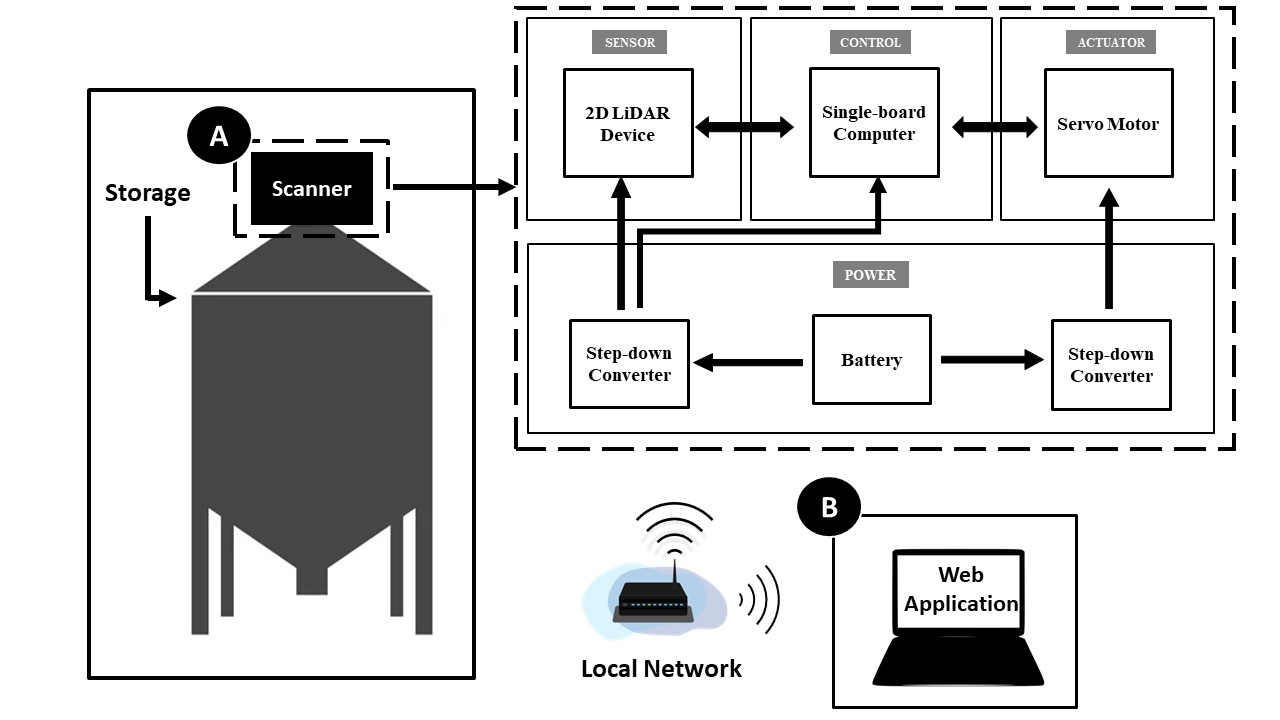
\includegraphics[width=1\textwidth]{Figures/system architecture}
	\caption{System Architecture Block Diagram: (A) 3D Point Cloud Scanner System, (B) Web Application}
	\label{ch3:fig:system-architecture}
\end{figure}

\begin{figure}[H]
	\centering
	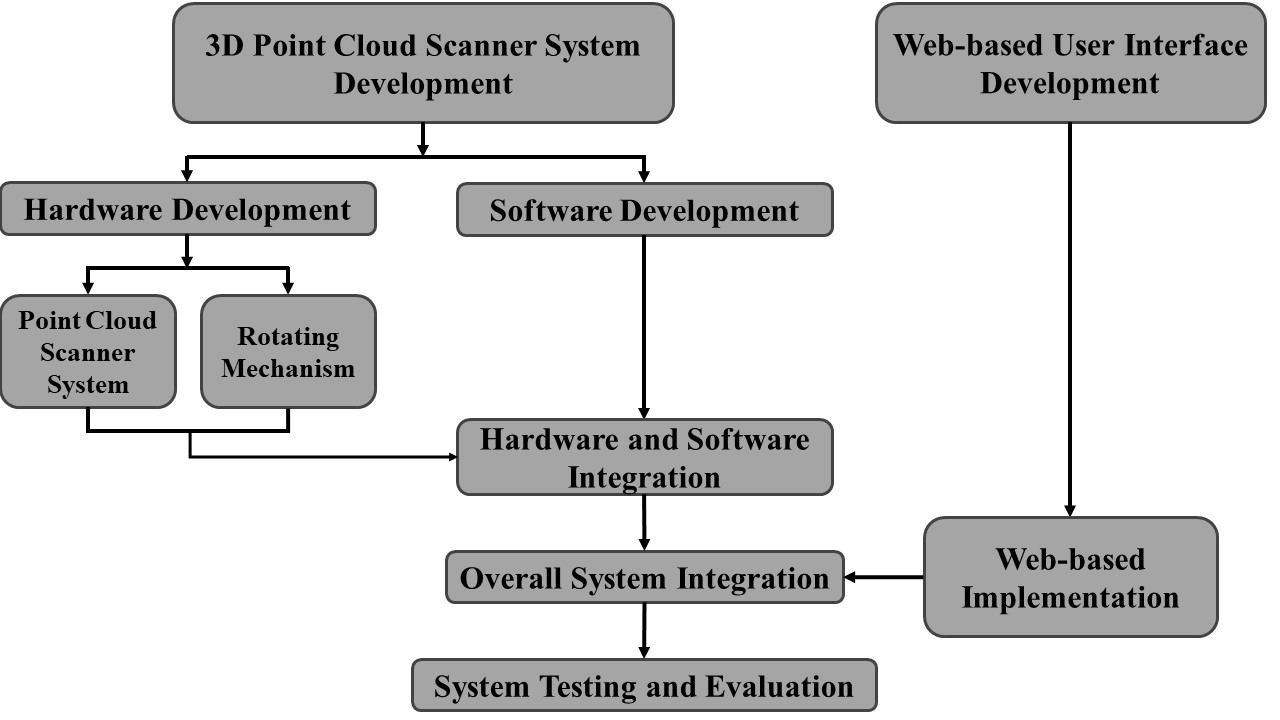
\includegraphics[width=1\textwidth]{Figures/system_development_process}
	\caption{System Development Process}
	\label{ch3:fig:system_development_process}
\end{figure}

\section{3D Point Cloud Scanner System Development}

The development flow chart of the system is shown in figure \ref{ch3:fig:3d-pcss_development_flow_chart} which composed of hardware and software development.

% In figure \ref{ch3:fig:components_of_3d-pcss}, the components of the point cloud scanner and rotating device are integrated to develop a 3D point cloud scanner system. These individual components are divided into four categories, as shown in figure \ref{ch3:fig:block-digram-connection}: sensor, control, actuator, and power. The double-headed arrow indicates a two-way communication from and to the control device. Lastly, the hardware design flow chart of the system is shown in figure \ref{ch3:fig:3d-pcss_development_flow_chart}.

\begin{figure}[H]
	\centering
	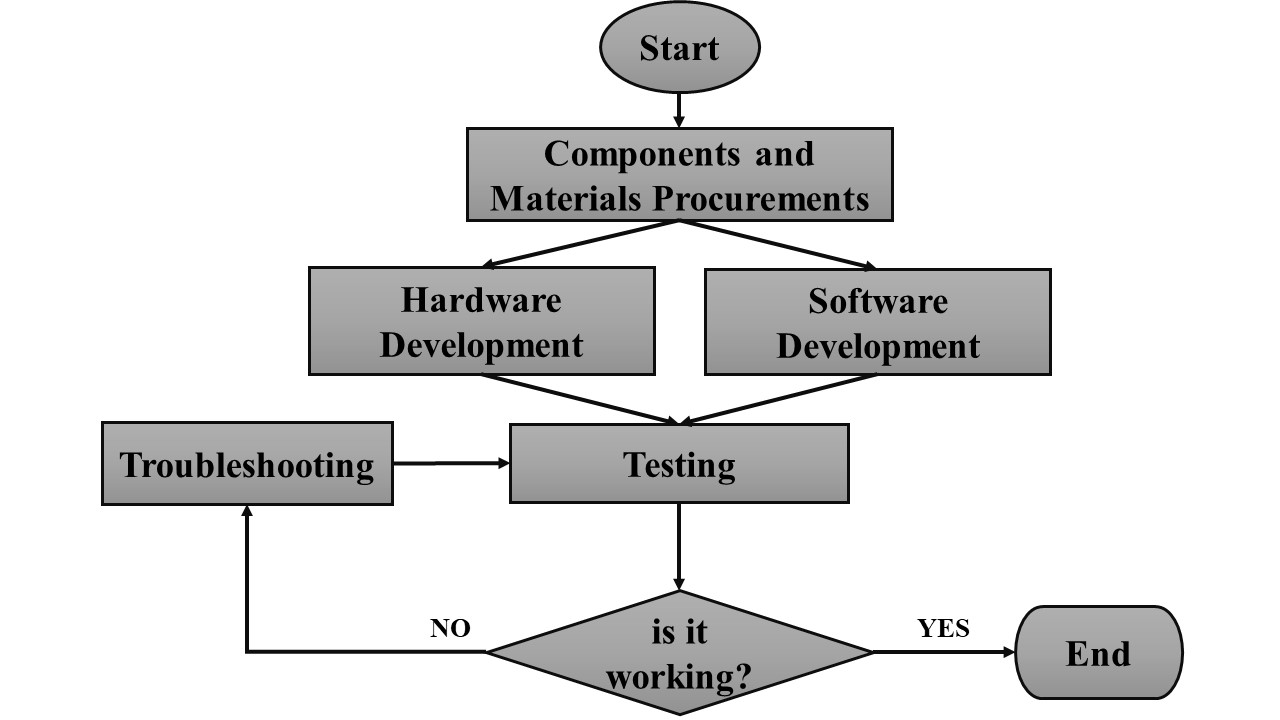
\includegraphics[width=1\textwidth]{Figures/hardware_flowchart}
	\caption{3D Point Cloud Scanner Development Flow Chart}
	\label{ch3:fig:3d-pcss_development_flow_chart}
\end{figure}

% \section{System Requirements Analysis}
% \label{ch3:sec:system_requirements_analysis}

% The development process of the study encompasses hardware, software, and web-based application design, followed by system integration and testing. As depicted in Figure \ref{ch3:fig:overall_system_setup_development} which is the proposed overall system setup, the study undertook the design and development of two distinct yet interconnected systems: the 3D Point Cloud Scanner (3D-PCSS), which is placed at the top of a storage bin, and the web-based application which is both connected to the local network. This overall system setup achieved by following a step by step development process which is illustrated in figure \ref{ch3:fig:system_development_process}, identifying hardware aspect which involves selecting and configuring the necessary components for data acquisition, processing, and communication. software development focuses on programming the processes to control hardware functionality and execute specific tasks. Meanwhile, web-based application design requires creating an interface for users to interact and data visualization. System integration involves bringing together these components and ensuring communication and functionality between them. Lastly, system testing and evaluation was conducted to validate the functionality, performance, and reliability of the developed systems through various testing procedures.

% \begin{figure}[H]
% 	\centering
% 	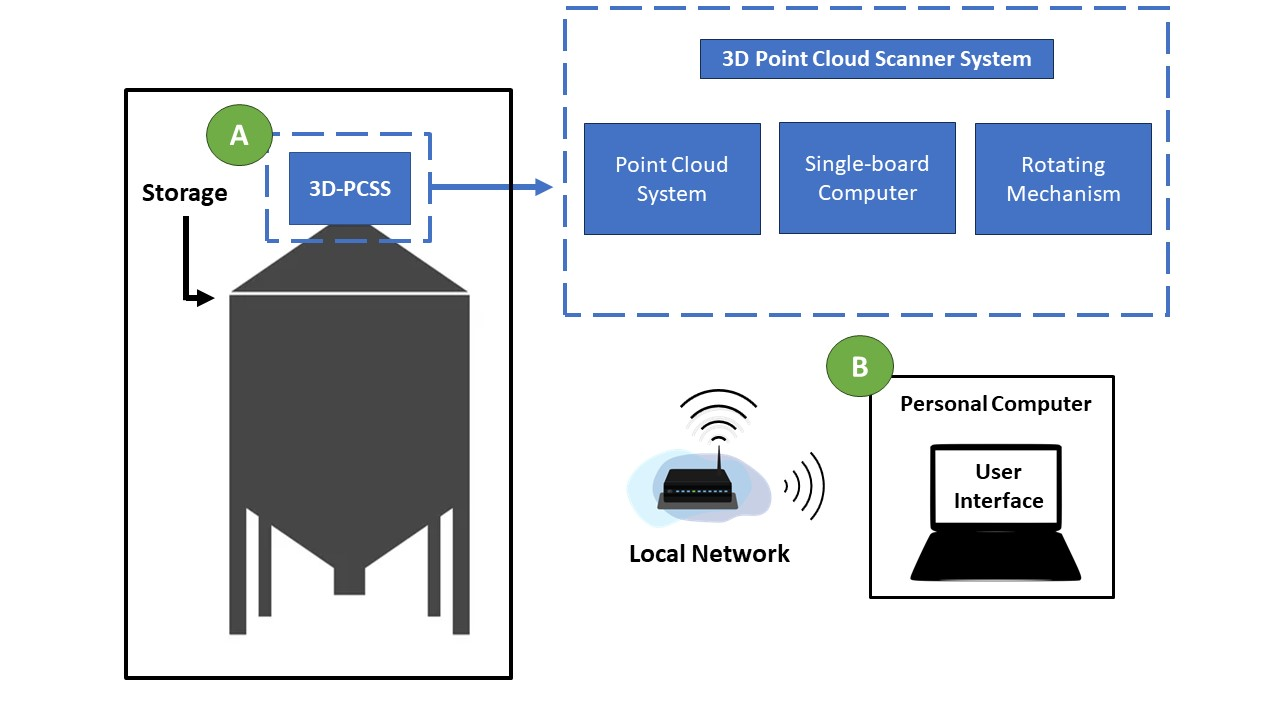
\includegraphics[width=1\textwidth]{Figures/system_analysis}
% 	\caption{Overall System Setup: (A) 3D-PCSS, (B) User Interface}
% 	\label{ch3:fig:overall_system_setup_development}
% \end{figure}

\subsection{Hardware Development}
\label{ch3:sec:hardaware_design}
The hardware components of the 3D Point Cloud Scanner System composed 2D LiDAR device and rotating mechanism.

\subsubsection{2D LiDAR Scanner}
The 2D LiDAR scanner comprises two major components: the 2D LiDAR Device and the single-board computer. The analysis of the hardware system requirements of 2D LiDAR Scanner in this study considers the following functionality:

\begin{itemize}
	\item A 2D LiDAR device capable of scanning within a 180-degree horizontal field of view.
	\item A 2D LiDAR device with a minimum range measurement capability of 10 meters.
	\item A single-board computer with a minimum CPU speed of 1.8GHz (64-bit architecture), 4GB of RAM, 5GB of disk space, and compatible with the required operating system.
\end{itemize}

% \begin{figure}[H]
% 	\centering
% 	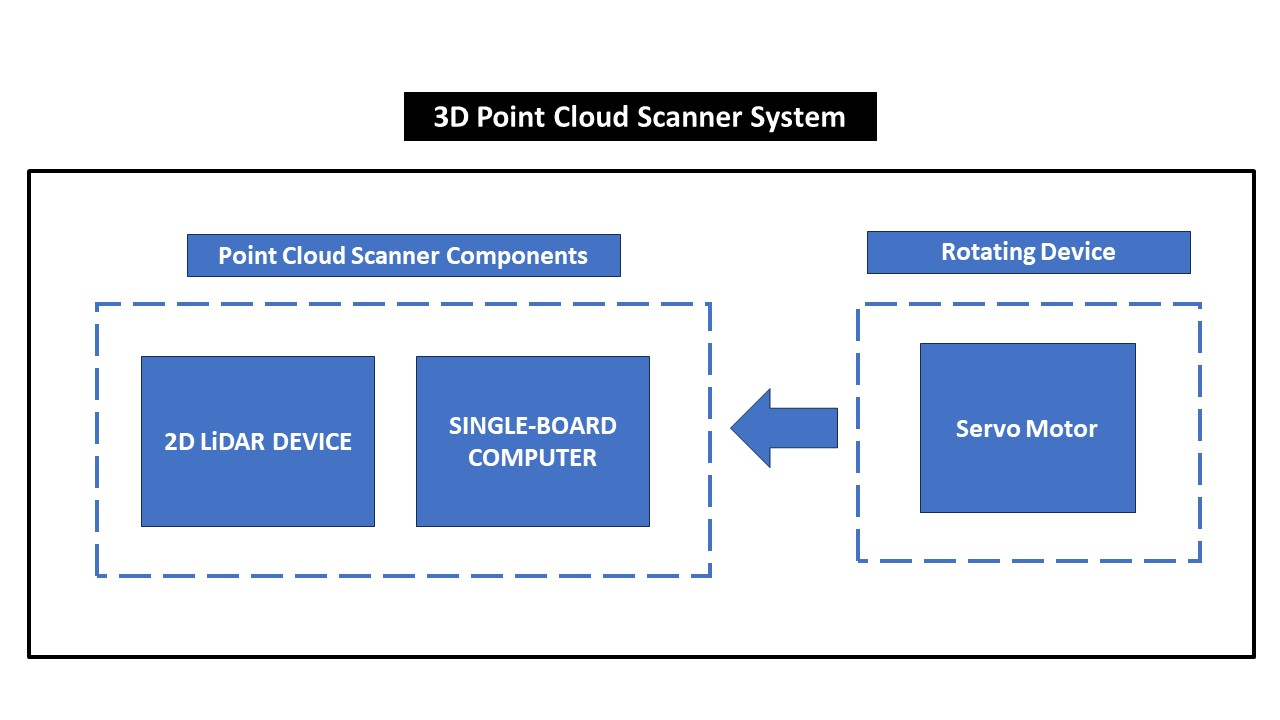
\includegraphics[width=1\textwidth]{Figures/3D-PCSS components}
% 	\caption{Hardware Components of the System}
% 	\label{ch3:fig:components_of_3d-pcss}
% \end{figure}

% The researcher will adopt the concept of tilting method using a 2D of-the-shelf LiDAR to acquire 3D point cloud data to minimize the cost compared to commercial 3D LiDAR. The hardware and physical components of 3D point cloud scanner are composed of three major components, the 2D LiDAR device, the tilting mechanism which include the fabricated holder for mechanical tilting and the motor for the rotation movement. In Figure \ref{ch3:fig:System Hardware Block Diagram}, the 3D point cloud scanner is placed at the top of the flour bin.

% \begin{figure}
% 	\centering
% 	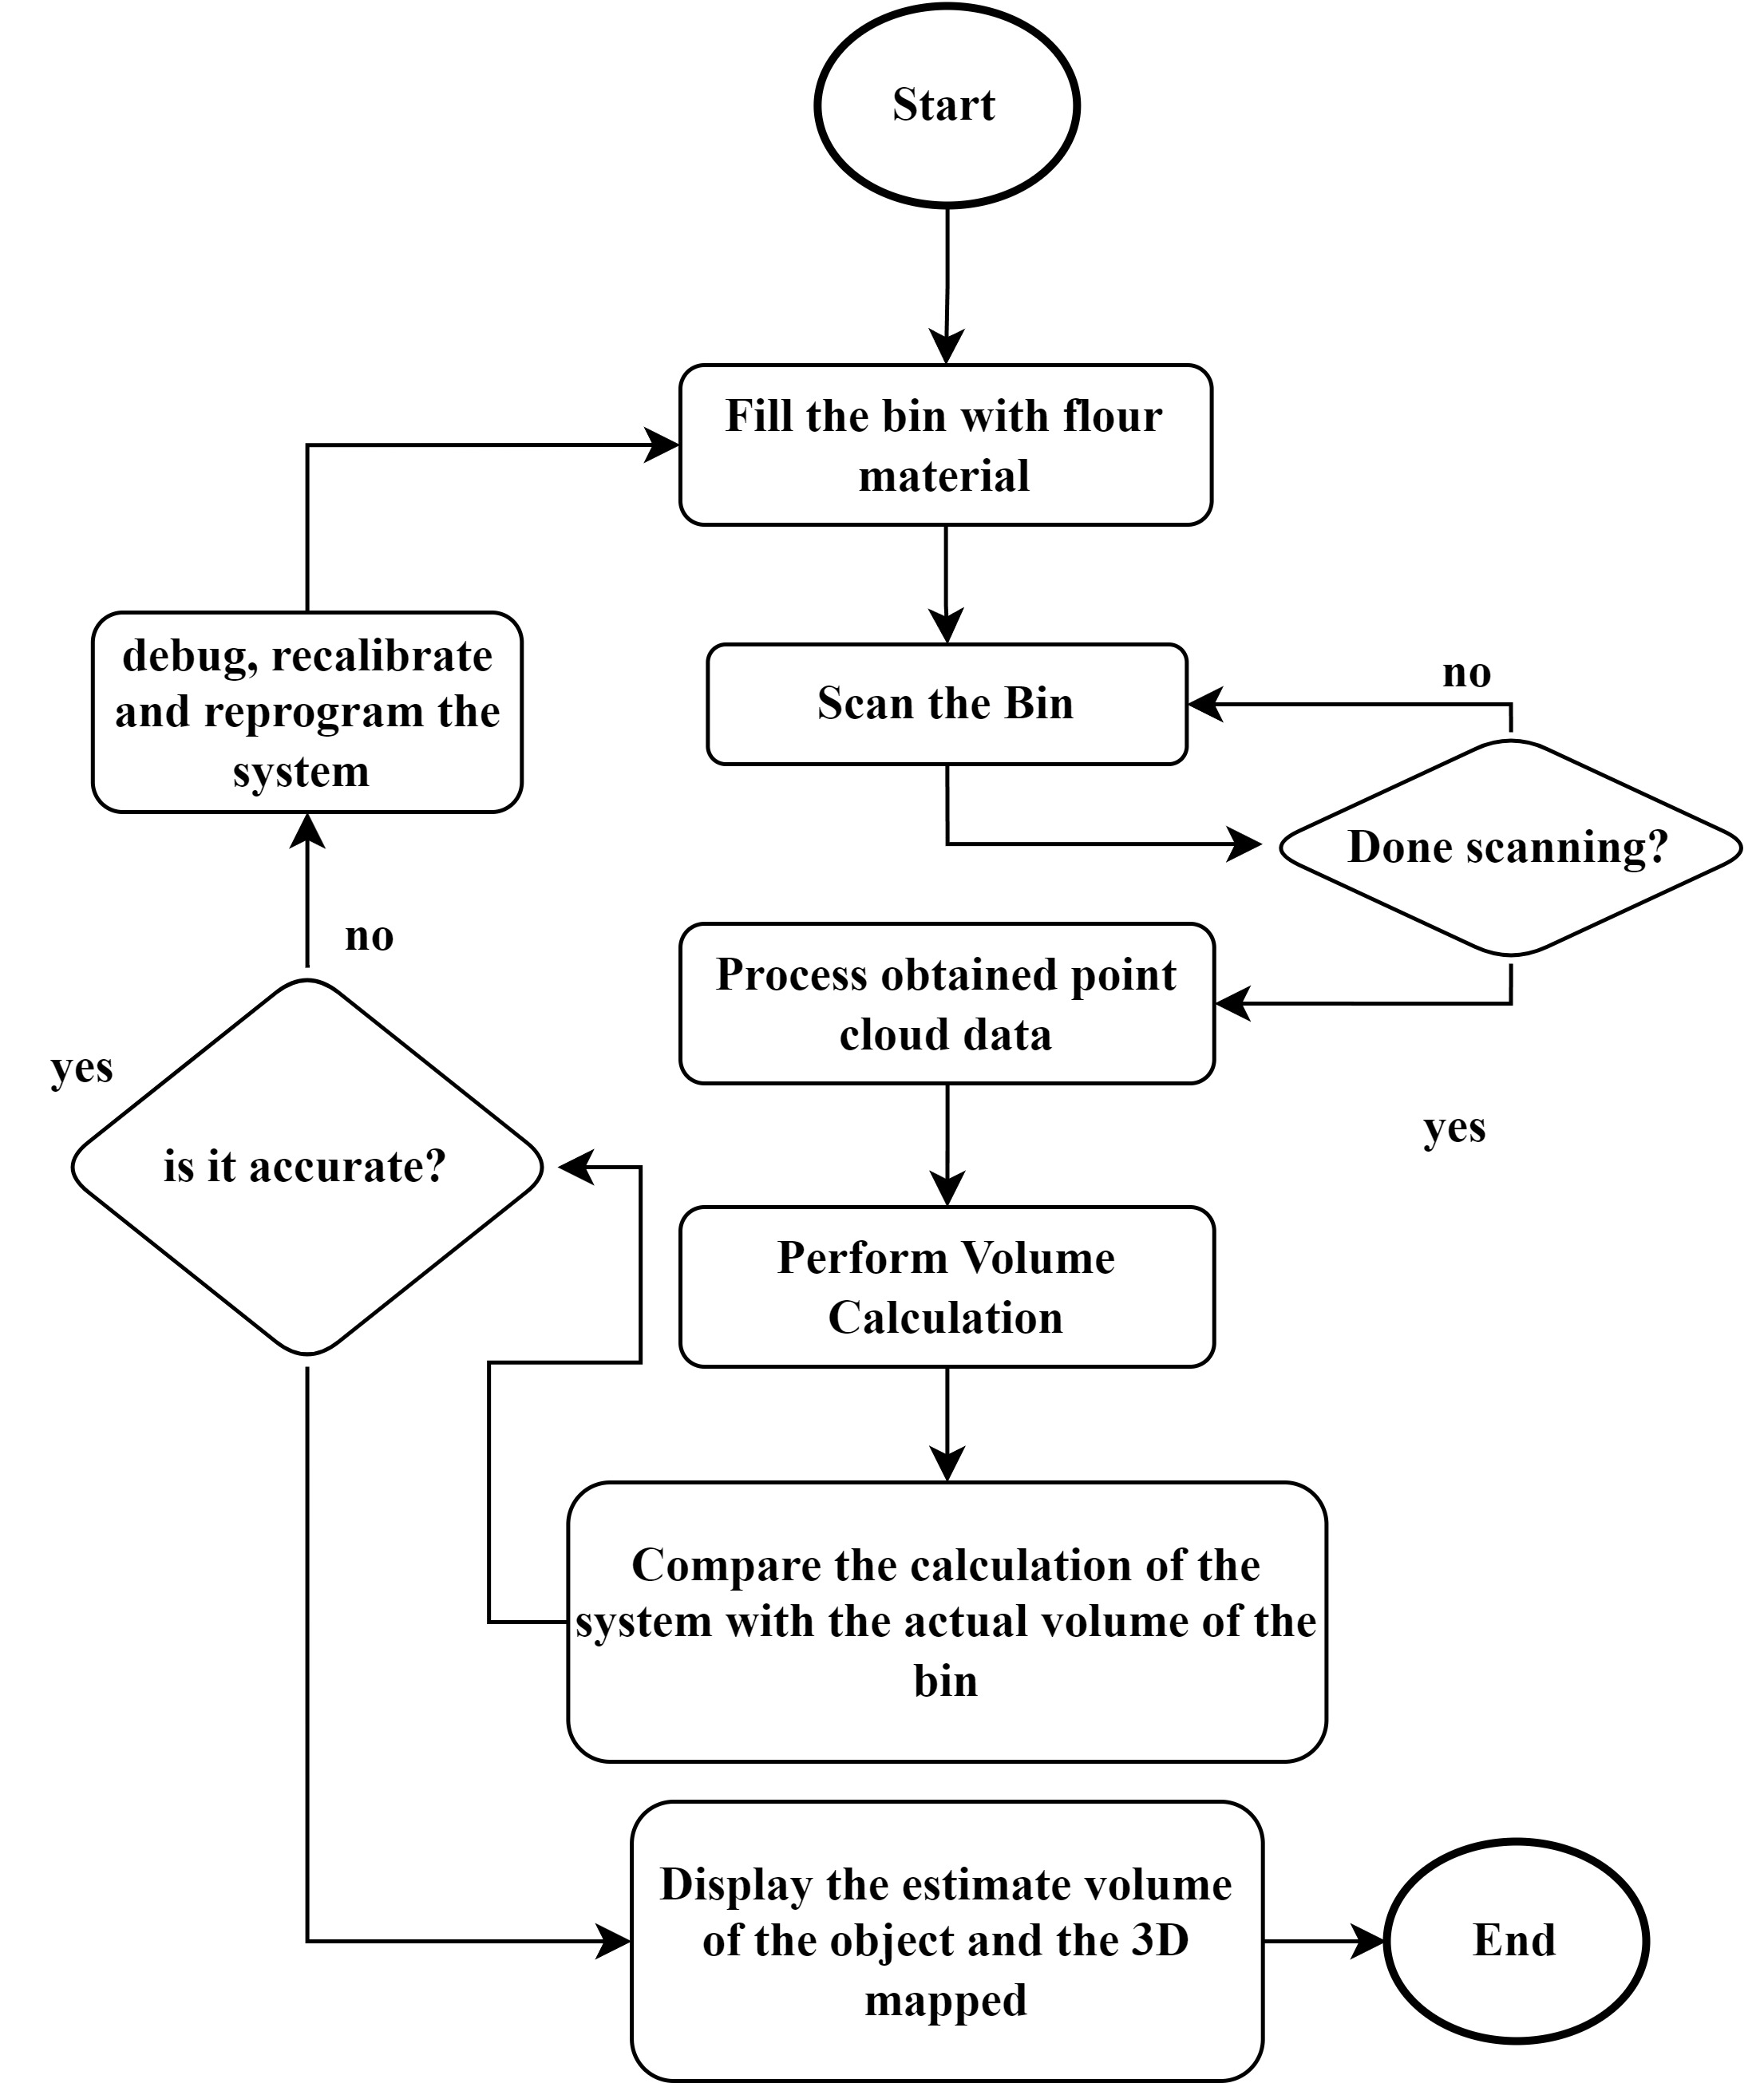
\includegraphics[width=0.9\textwidth]{Figures/general-flowchart-of-the-system-2.jpg}
% 	\caption{General Flowchart of the System}
% 	\label{ch3:fig:General flowchart of the system}
% \end{figure}

% \subsection{3D Point Cloud Scanner Design (3D-PCSS)}
% \label{ch3:subsec:3d_point_cloud_scanner_design}

% The 3D-PCSS in this study considers the following design and functionality:
% \begin{itemize}
% 	\item Based on low-cost 2D LiDAR device.
% 	\item Compact and portable for simplified installation.
% 	\item Support for connecting to a local network for remote data visualization and monitoring.
% 	\item Utilizing Robot Operating System (ROS) and Point Cloud Library (PCL) for adaptability development.
% \end{itemize}

% To achieve the design and functionality of the system mentioned, the development process, components and integration is discussed in the following section

% \subsubsection{Point Cloud Scanner System}

% Point cloud devices, such as LiDAR (Light Detection and Ranging), offer exceptional accuracy in acquiring distance measurements over considerable distances. LiDAR systems emit laser pulses and measure the time it takes for these pulses to return after bouncing off objects in the environment. This technology enables the creation of highly detailed and accurate three-dimensional point clouds, which represent the surfaces and structures within the scanned area. Even low-cost LiDAR options are available in the market, making this technology accessible for various applications and budgets.

% The point cloud scanner system in this study used a low-cost 2D LiDAR device controlled with single-board computer (SBC) for its computing functionality.

\subsubsection{Rotating Mechanism}

The rotating mechanism design which is attached to the 2D LiDAR in this study is based on the methodology outlined in a previous research conducted by \citet{clar2022}. This prior study served as a foundational framework for the development of the rotating 2D LiDAR system in this study, providing into the integration of a pan-tilt unit (PTU) with a 2D LiDAR scanner to enable three-dimensional point cloud scanning.

The functionality of the rotating device consider in this study has the following functionality:

\begin{itemize}
	\item The rotating device can rotate a minimum angle from 0 of 180 degree.
	\item The rotating device has a minimum angular resolution of $\le1$ degree.
\end{itemize}

% The servo motor utilized in this study is compatible with a Software Development Kit (SDK), which includes configurations for integration with the Robot Operating System (ROS). This feature enables communication and control of the servo motor within the ROS ecosystem, allowing for flexible and efficient development of robotic systems. This feature enables the LiDAR and Servo to communicate and synchronize, figure \ref{} illustrates the servo attached to the 2D LiDAR device to add additional axis. The figure shows the respective scan angle direction of the LiDAR and servo motor. The curial part of in this process is the synchronization process which in this study developed as shows in figure \ref{ch3:fig:servo_lidar_comm}. \\

% \begin{algorithm}[]
% 	\caption{LDA}
% 	\label{ch3:algo:servo_and_lidar}
% 	\begin{algorithmic}[1]
% 		\FOR{$d$}
% 		\STATE{
% 			\FOR{$k\in\{1,...,K\}$}
% 			\STATE{Generate$\beta_k=(\beta_{k_1},...,\beta_{k,V})^T \sim Dirichlet(\cdot\vert\eta)$}
% 			\ENDFOR
% 		}
% 		\ENDFOR
% 	\end{algorithmic}
% \end{algorithm}

Figure \ref{ch3:fig:servo_lidar_comm} provides an illustration of the servo's attachment to the 2D LiDAR device, enabling an additional axis of movement. It also demonstrates the respective scan angle directions of the LiDAR and the movement direction of the servo motor. This synchronization method is further detailed in flow chart shown in Figure \ref{ch3:fig:scan_and_movement_direction}. After the LiDAR scans from 0 to 180 degrees, the system sends a command to the servo to move to the next angle until it reaches the end angle. %Additionally, the block diagram connection of the overall hardware system is presented in Figure \ref{ch3:fig:block-digram-connection}.
\\
\begin{figure}[H]
	\centering
	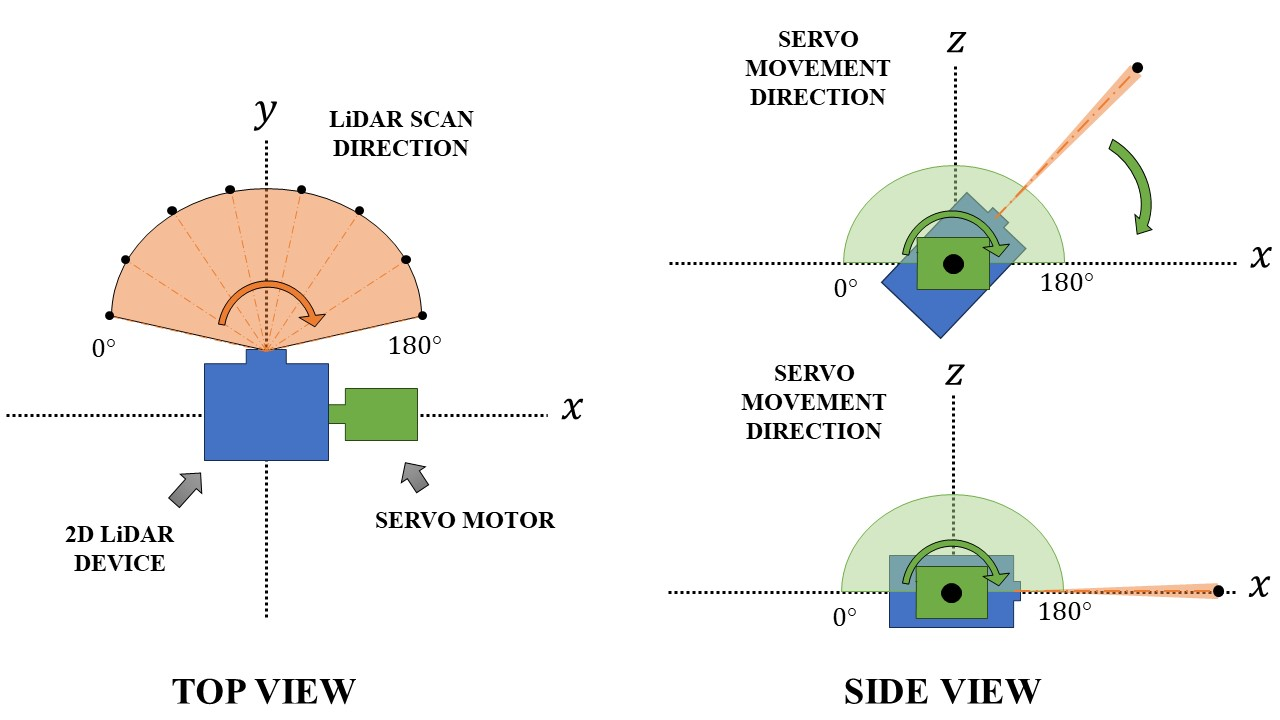
\includegraphics[width=1\textwidth]{Figures/scan_direction_of_lidar_and_servo}
	\caption{Scan Direction of LiDAR and Movement Direction of the Servo}
	\label{ch3:fig:servo_lidar_comm}
\end{figure}


\begin{figure}[H]
	\centering
	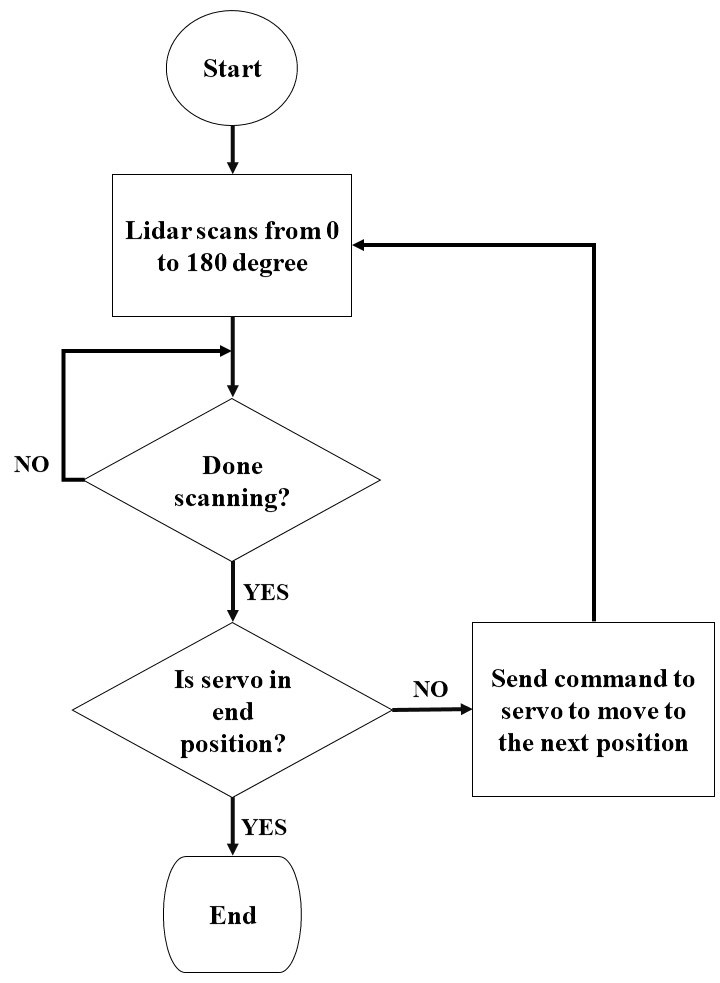
\includegraphics[width=0.8\textwidth, height=0.9\textwidth]{Figures/lidar_servo_sync}
	\caption{Synchronization Process of LiDAR and Servo}
	\label{ch3:fig:scan_and_movement_direction}
\end{figure}

% \begin{figure}[H]
% 	\centering
% 	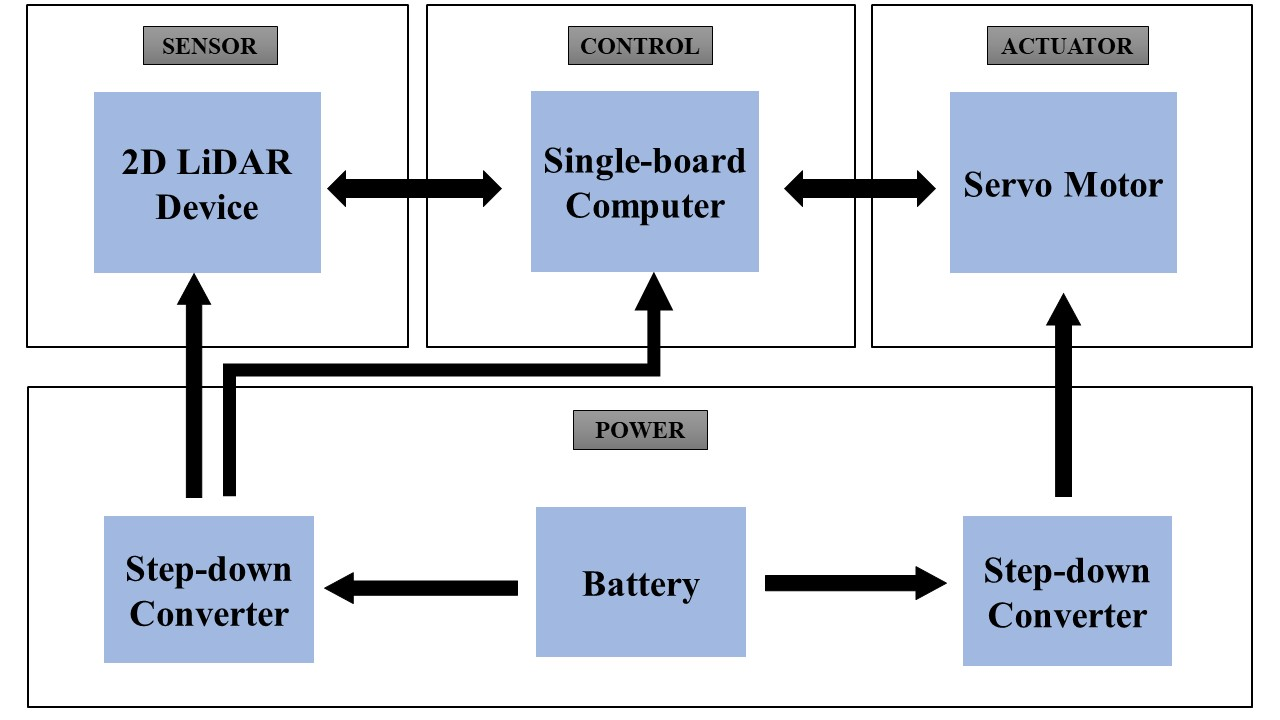
\includegraphics[width=1\textwidth]{Figures/components-block-diagram}
% 	\caption{Block Diagram Connection of the Components}
% 	\label{ch3:fig:block-digram-connection}
% \end{figure}

% \subsubsection*{Point Cloud Scanner System}

% Point cloud devices, such as LiDAR (Light Detection and Ranging), offer exceptional accuracy in acquiring distance measurements over considerable distances. LiDAR systems emit laser pulses and measure the time it takes for these pulses to return after bouncing off objects in the environment. This technology enables the creation of highly detailed and accurate three-dimensional point clouds, which represent the surfaces and structures within the scanned area. Even low-cost LiDAR options are available in the market, making this technology accessible for various applications and budgets.

% The point cloud scanner system in this study used a low-cost 2D LiDAR device controlled with single-board computer (SBC) for its computing functionality.

% \subsubsection*{Rotating Mechanism}

% The rotating mechanism design which is attached to the 2D LiDAR in this study is based on the methodology outlined in a previous research conducted by \citet{clar2022}. This prior study served as a foundational framework for the development of the rotating 2D LiDAR system in this study, providing into the integration of a pan-tilt unit (PTU) with a 2D LiDAR scanner to enable three-dimensional point cloud scanning. By employment the principles and techniques conducted in \citet{clar2022}, the current study aims to further refine and enhance the performance of the rotating 2D LiDAR system for its intended application and also address the problem encountered in the previous study.

% % The servo motor utilized in this study is compatible with a Software Development Kit (SDK), which includes configurations for integration with the Robot Operating System (ROS). This feature enables communication and control of the servo motor within the ROS ecosystem, allowing for flexible and efficient development of robotic systems. This feature enables the LiDAR and Servo to communicate and synchronize, figure \ref{} illustrates the servo attached to the 2D LiDAR device to add additional axis. The figure shows the respective scan angle direction of the LiDAR and servo motor. The curial part of in this process is the synchronization process which in this study developed as shows in figure \ref{ch3:fig:servo_lidar_comm}. \\

% The servo motor used in this study is compatible with a Software Development Kit (SDK) that includes configurations for integration with the Robot Operating System (ROS). This compatibility allows for communication and control of the servo motor within the ROS environment, facilitating the development of flexible and efficient robotic systems.

% By employing this feature, the LiDAR and servo can communicate and synchronize. Figure \ref{ch3:fig:scan_and_movement_direction} illustrates how the servo is attached to the 2D LiDAR device to add an additional axis of movement. The figure also depicts the respective scan angle directions of the LiDAR and the movement direction servo motor.

% Synchronization is a crucial aspect of this process. The synchronization method developed in this study is detailed in Figure \ref{ch3:fig:servo_lidar_comm}.

% % \begin{algorithm}[]
% % 	\caption{LDA}
% % 	\label{ch3:algo:servo_and_lidar}
% % 	\begin{algorithmic}[1]
% % 		\FOR{$d$}
% % 		\STATE{
% % 			\FOR{$k\in\{1,...,K\}$}
% % 			\STATE{Generate$\beta_k=(\beta_{k_1},...,\beta_{k,V})^T \sim Dirichlet(\cdot\vert\eta)$}
% % 			\ENDFOR
% % 		}
% % 		\ENDFOR
% % 	\end{algorithmic}
% % \end{algorithm}

% \begin{figure}[H]
% 	\centering
% 	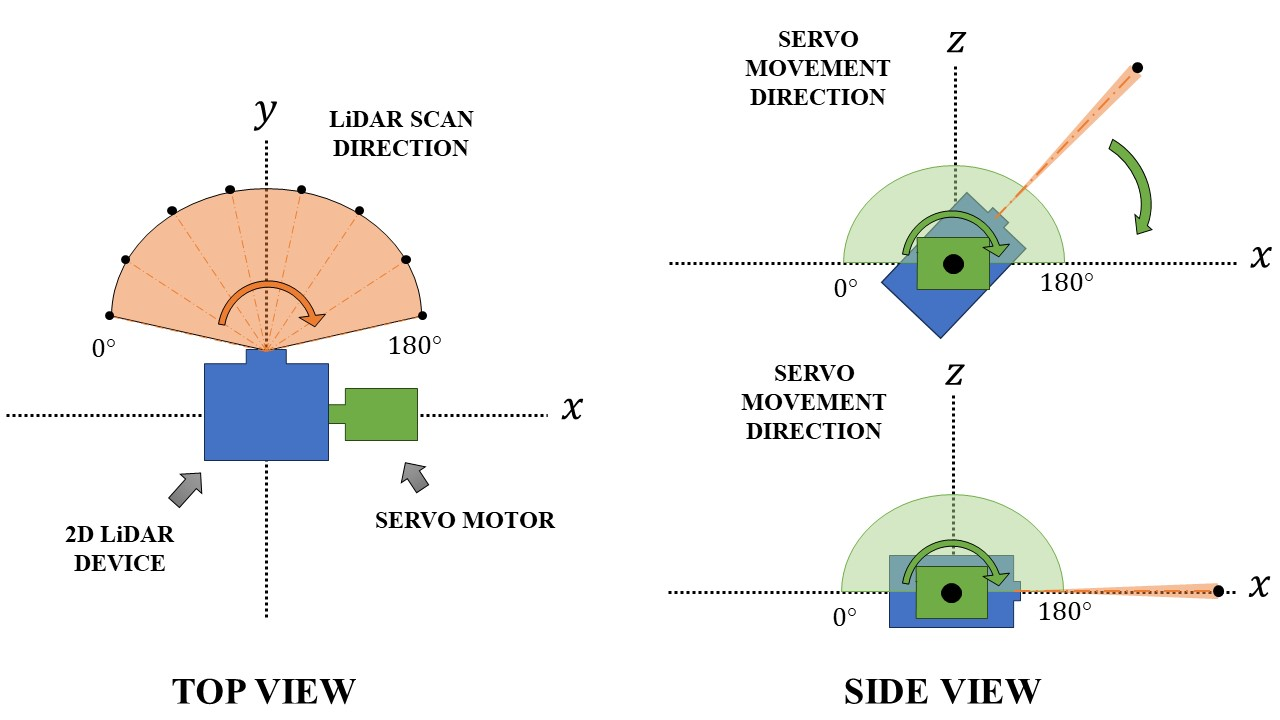
\includegraphics[width=1\textwidth]{Figures/scan_direction_of_lidar_and_servo}
% 	\caption{Scan Direction of LiDAR and Movement Direction of the Servo}
% 	\label{ch3:fig:servo_lidar_comm}
% \end{figure}

% \begin{figure}[H]
% 	\centering
% 	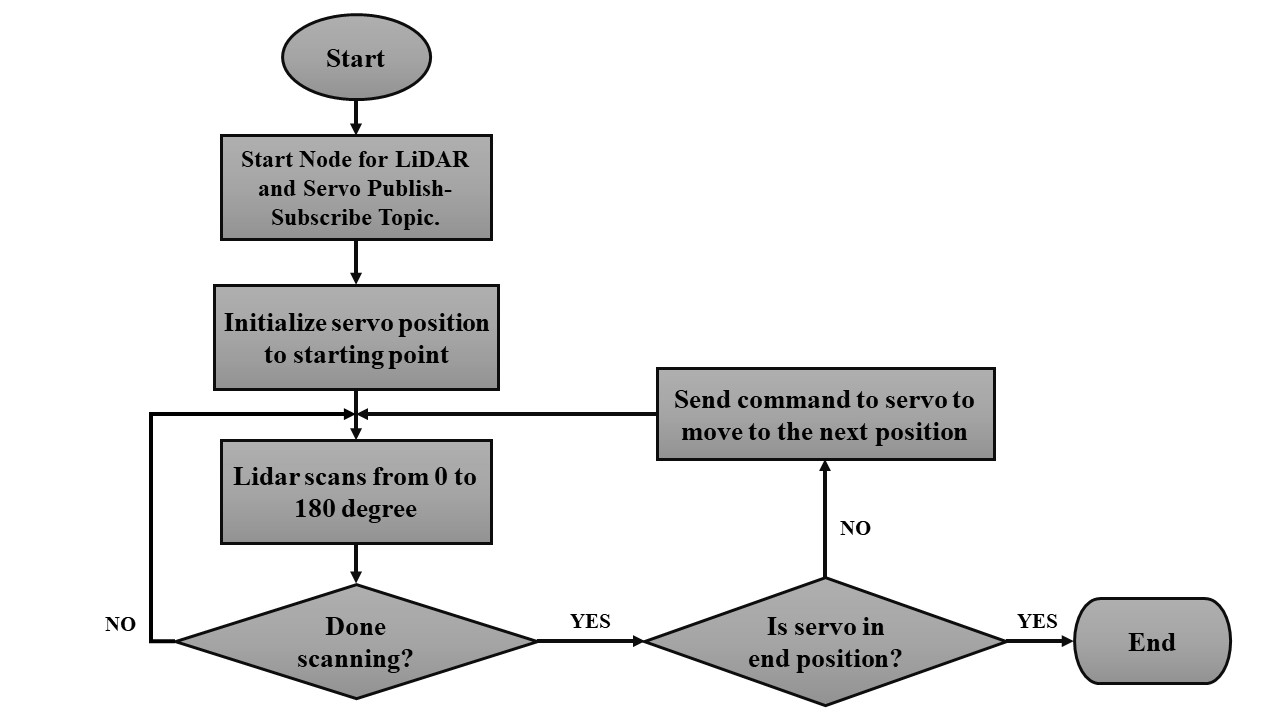
\includegraphics[width=1\textwidth]{Figures/servo_lidar_comm}
% 	\caption{Synchronization Process of LiDAR and Servo}
% 	\label{ch3:fig:scan_and_movement_direction}
% \end{figure}

% In figure \ref{ch3:fig:components_of_3d-pcss}, the components of the point cloud scanner and rotating device are integrated to develop a 3D point cloud scanner system. These individual components are divided into four categories, as shown in figure \ref{ch3:fig:block-digram-connection}: sensor, control, actuator, and power. The double-headed arrow indicates a two-way communication from and to the control device. Lastly, the hardware design flow chart of the system is shown in figure \ref{ch3:fig:3d-pcss_development_flow_chart}.

% \begin{figure}[H]
% 	\centering
% 	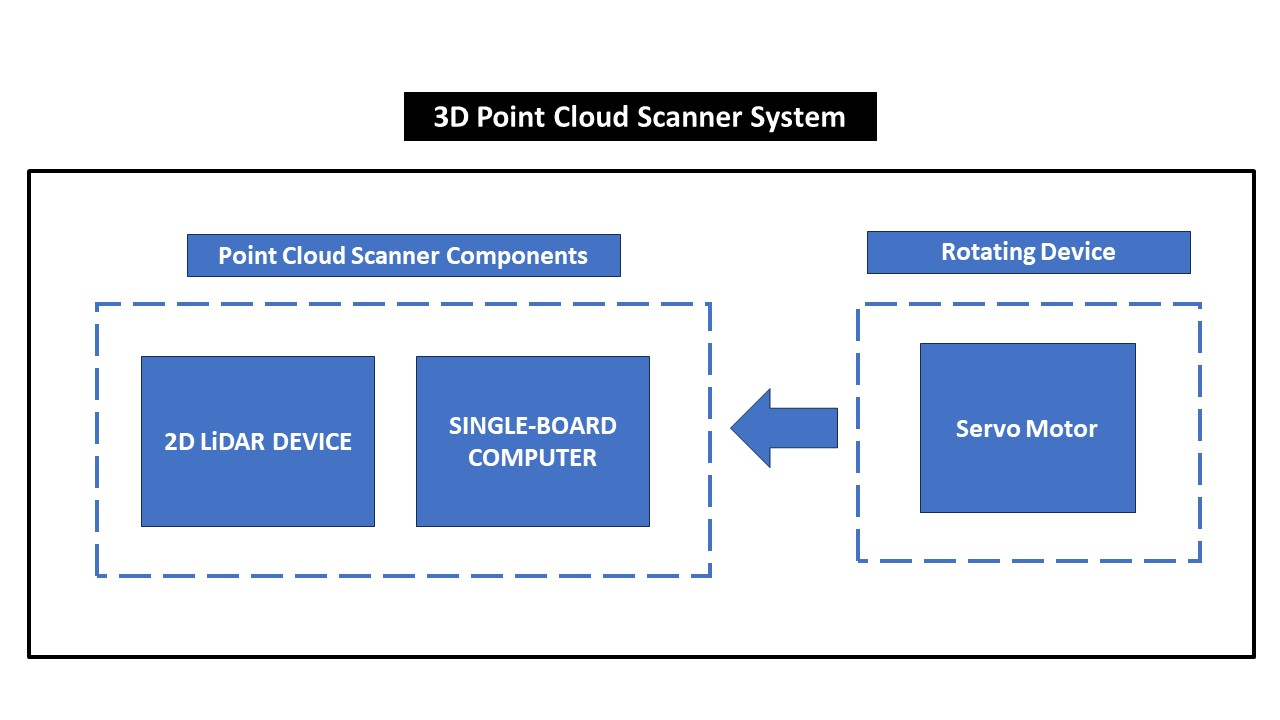
\includegraphics[width=1\textwidth]{Figures/3D-PCSS components}
% 	\caption{Major Components of 3D-PCSS}
% 	\label{ch3:fig:components_of_3d-pcss}
% \end{figure}

% \begin{figure}[H]
% 	\centering
% 	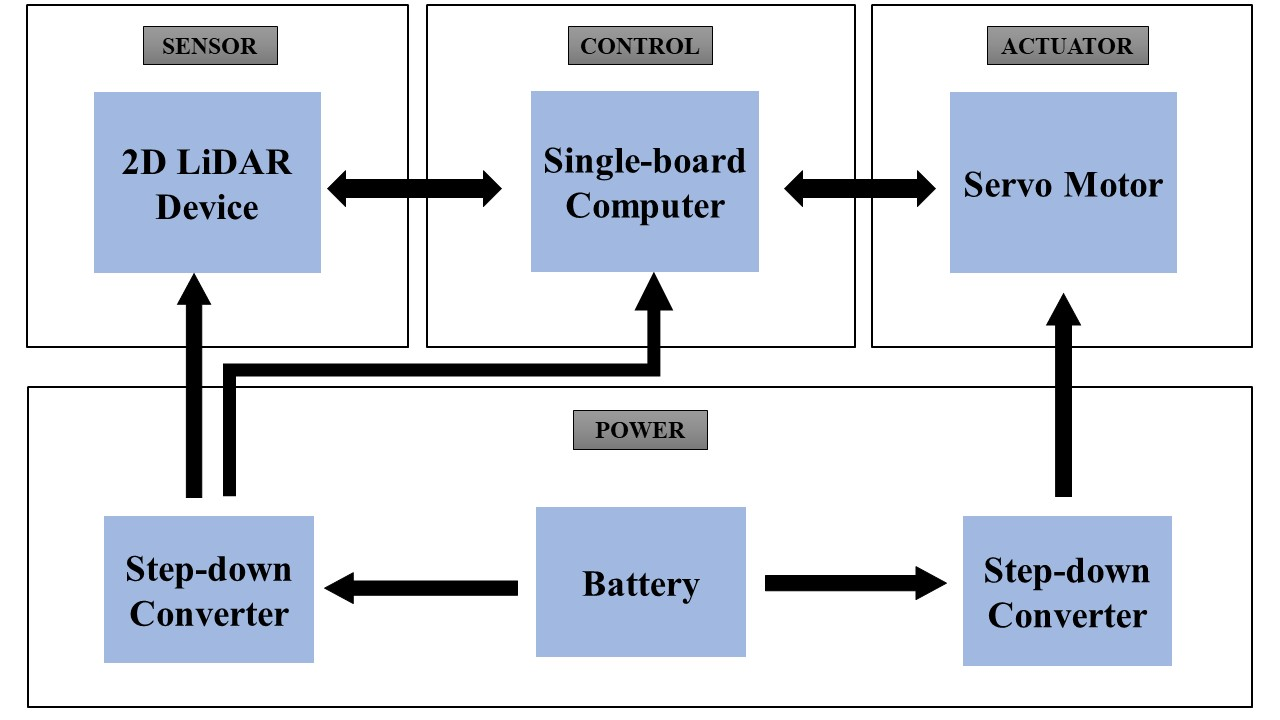
\includegraphics[width=1\textwidth]{Figures/components-block-diagram}
% 	\caption{Block Diagram Connection of the Components}
% 	\label{ch3:fig:block-digram-connection}
% \end{figure}


% \begin{figure}[H]
% 	\centering
% 	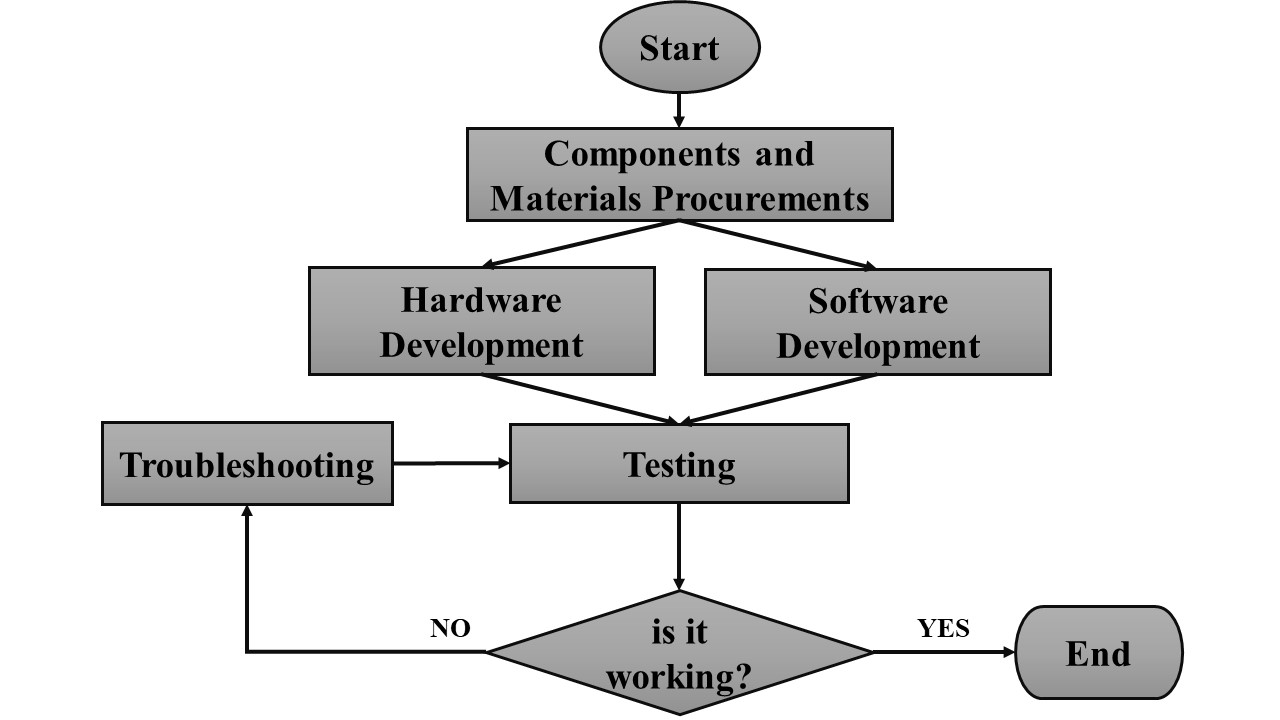
\includegraphics[width=0.8\textwidth]{Figures/hardware_flowchart}
% 	\caption{Hardware Design Flow Chart}
% 	\label{ch3:fig:3d-pcss_development_flow_chart}
% \end{figure}

% \subsection{Data Gathering}
% For the data gathering of the raw point cloud, all the major hardware of the system will be assemble and integrate as shown in Figure \ref{ch3:fig:System Hardware Block Diagram}. The scanned data from the 2D LiDAR sensor will be received by small computer which is Raspberry Pi for the processing of the raw data. This small computer is connected to the internet in order to control remotely by the personal laptop. Different scanning procedure will be performed to gather point cloud data.

% \begin{figure}[H]
% 	\centering
% 	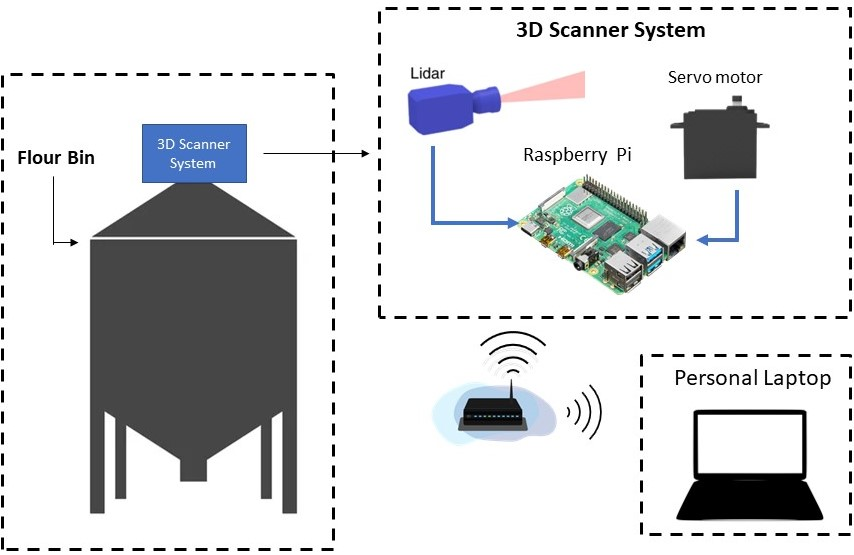
\includegraphics[width=0.9\textwidth]{Figures/system-hardware-block-diagram.jpg}
% 	\caption{System Hardware Block Diagram}
% 	\label{ch3:fig:System Hardware Block Diagram}
% \end{figure}

\subsection{Software Development}
\label{ch3:subsec:software-development}

Software development plays a crucial role in the overall development of the 3D Point Cloud Scanner System. The flow of the different software processes developed in this study is shown in figure \ref{ch3:fig:software-development}  The system was designed to initialize all necessary components, including nodes and connection, immediately upon power-up. This ensures seamless operation and also establish connection with the developed web application for user interaction. Figure \ref{ch3:fig:nodes-topics-relationships} shows the different nodes, topics and their relationship of the software of the system. \\

\begin{figure}[H]
	\centering
	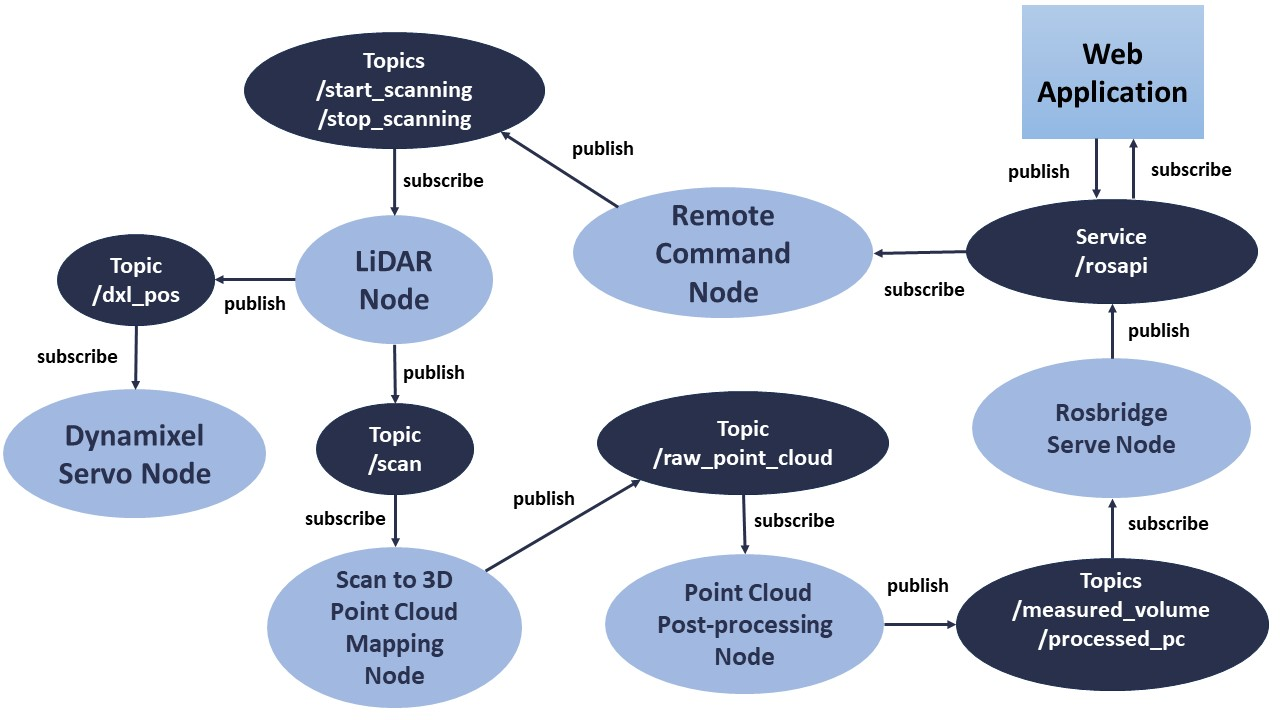
\includegraphics[width=1\textwidth]{Figures/nodes-topics-relationship}
	\caption{Nodes, Topics and their Relationships}
	\label{ch3:fig:nodes-topics-relationships}
\end{figure}

\begin{figure}[H]
	\centering
	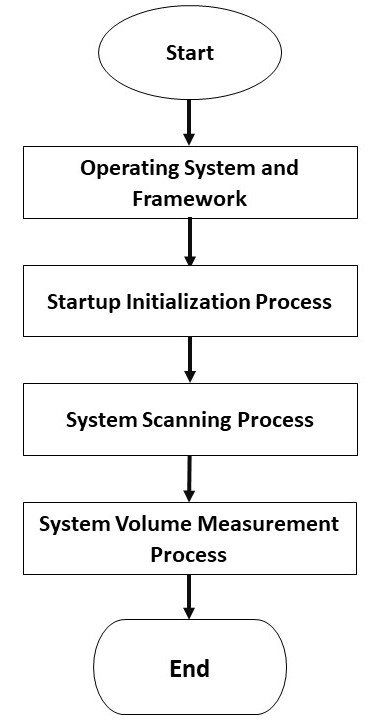
\includegraphics[width=0.5\textwidth, height=0.9\textwidth]{Figures/software-development}
	\caption{Flow Chart of the Different Software Processes}
	\label{ch3:fig:software-development}
\end{figure}

\subsubsection{Operating System and Frameworks}

In this study, the single-board computer (SBC) used in the 3D Point Cloud Scanner System requires an appropriate OS and frameworks to support the execution of firmware and software components. Linux-based operating systems, such as Ubuntu, is commonly chosen for SBCs due to its reliability, flexibility, and extensive community support. This OS option provide a stable platform for running Robot Operating System (ROS) nodes and managing system resources effectively, thus, was utilized in this study. ROS framework was also utilized in this study to develop a publish-subscribe relationship between ROS nodes. Lastly, Point Cloud Library (PCL) serves in this study as a fundamental library being used for processing and analyzing point cloud data. PCL provides a comprehensive set of algorithms and tools for tasks such as point cloud registration, filtering and computational geometry to name a few.

\subsubsection{Startup Initialization Process}
Roscore and rosgridge are the two essential cores that used in the software of 3D-PCSS. These cores typically need to be executed manually through the command-line interface (CLI) or desktop environment terminal to run and process data, or to initiate other nodes and do specific tasks. In this study a custom service file was developed to automate and start these nodes after the system is turn on. This file is created using Linux systemd to configure and instantly run the cores. As described in figure \ref{ch3:fig:software_system_process}, after the system is energize, it initializes essential nodes and enter in idle mode waiting for an external command coming from the web application. The system remain in idle mode unless turnoff. The development of software processes, including the choice of operating system and frameworks is outlined in this section. \\
\begin{figure}[H]
	\centering
	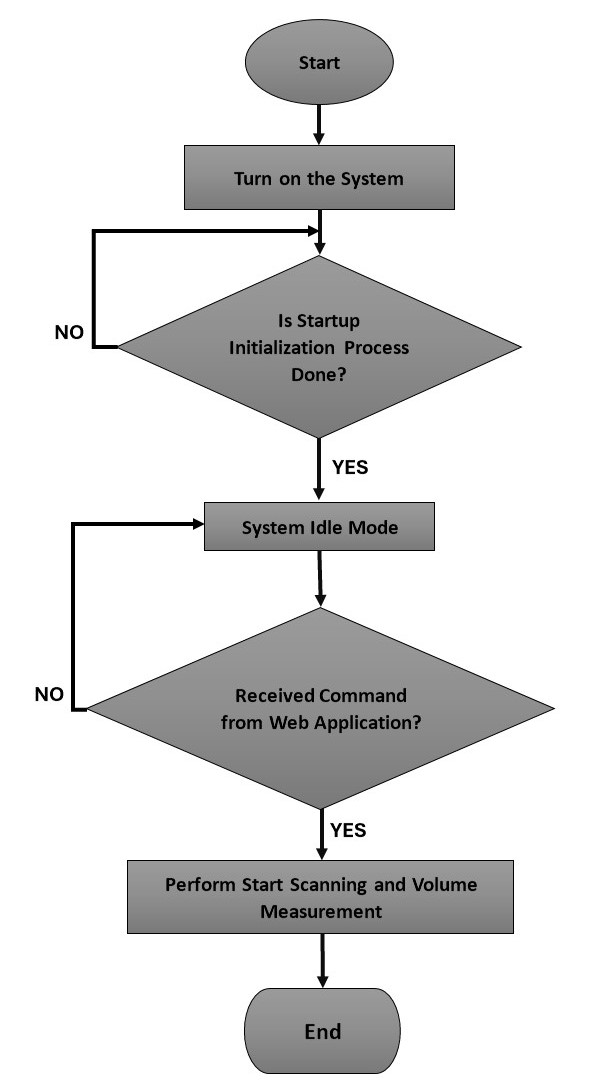
\includegraphics[width=0.7\textwidth, height=0.7\textheight]{Figures/software_system_process}
	\caption{System Idle Mode Process Flow Chart}
	\label{ch3:fig:software_system_process}
\end{figure}

% The Raspberry Pi will receive the scanned raw data coming from the 3D point cloud scanner. This data will be processed in different stages to produced desired output, such as point cloud pre-processing (formatting, converting, clustering, and cleansing) and post-processing (e.g., 3D mapping and volume measurement). Various platforms and frameworks nowadays are available to ease the handling of these massive raw data, thus, formatting the data to a desired platform must be perform. Typically, the value of raw data coming from the LiDAR sensor is not directly a point cloud data but rather a value of the distance between the sensor and the reflected nearest object in a particular direction, therefore, the data is converted into point cloud which composed of x, y, and z values. The Equation \eqref{ch3:eq:x-point}, \eqref{ch3:eq:y-point}, and \eqref{ch3:eq:z-point} is conversion of polar coordinates (distance, angle) to cartesian coordinates x, y, and z, respectively, in a 3D coordinate system.

% \begin{equation}
% 	x_{point_{i}} = \ \sin(i) \cdot d \
% 	\label{ch3:eq:x-point}
% \end{equation}
% \begin{equation}
% 	y_{point_{i}} = \ \cos(\pi) \cdot \cos(i) \cdot d \
% 	\label{ch3:eq:y-point}
% \end{equation}
% \begin{equation}
% 	z_{point_{i}} = \ -\cos(i) \cdot \sin(\pi) \cdot d \
% 	\label{ch3:eq:z-point}
% \end{equation}

% Where:

% \indent \indent i = scan angle of the scanner

% \indent \indent d = the distance point of the emitted pulse by the LiDAR (meter)

\subsubsection{System Scanning Process}
As described in conceptual framework shown in figure \ref{fig:conceptual-framework}, the system is placed at the top of the storage bin. Once the system receive a command from the web application, it will start scanning the inside of the storage bin and acquiring ranges values from the LiDAR as discussed in figure \ref{ch3:fig:software_system_process} else the system enters idle mode. The study developed a ros nodes that handle different processes such as initialization of the LiDAR device and servo motor, establishing a publish-subscribe relationship between these devices, and the conversion of LiDAR range scan data to point cloud data. The servo motor used in this study is compatible with a Software Development Kit (SDK) that includes configurations for integration with the Robot Operating System (ROS). The raw scan data from the LiDAR are typically range values of the return pulses. These range values enters different stages of pre-processes to be mapped in two- or three-dimensional Euclidean space to create a point cloud data and use for further post-processing. The flow of the processes from initialization to mapped point cloud data is illustrated in this figure \ref{ch3:fig:scanning-to-pc-flow-chart}. The method used in this study for processing the ranges values gathered from the LiDAR device is described in the figure \ref{ch3:fig:point_cloud_conversion} which was discussed in the theoretical framework.  $\rho$ translates to the distance from the origin $(0,0,0)$, which is the in our case the LiDAR, and this distance is measured as meter. The angle $\theta$ is the rotation around the z-axis in the xy-plane. The angle $\phi$ is the tilt of the radius vector from the positive z-axis, it goes from 0 degree at the positive z-axis down to 90 degree at the xy-plane and all the way down to 180 degree on the negative z-axis. Equation \ref{ch3:eq:x}, \ref{ch3:eq:y} and \ref{ch3:eq:z} shows the X, Y, and Z conversion formula respectively.

\begin{figure}[H]
	\centering
	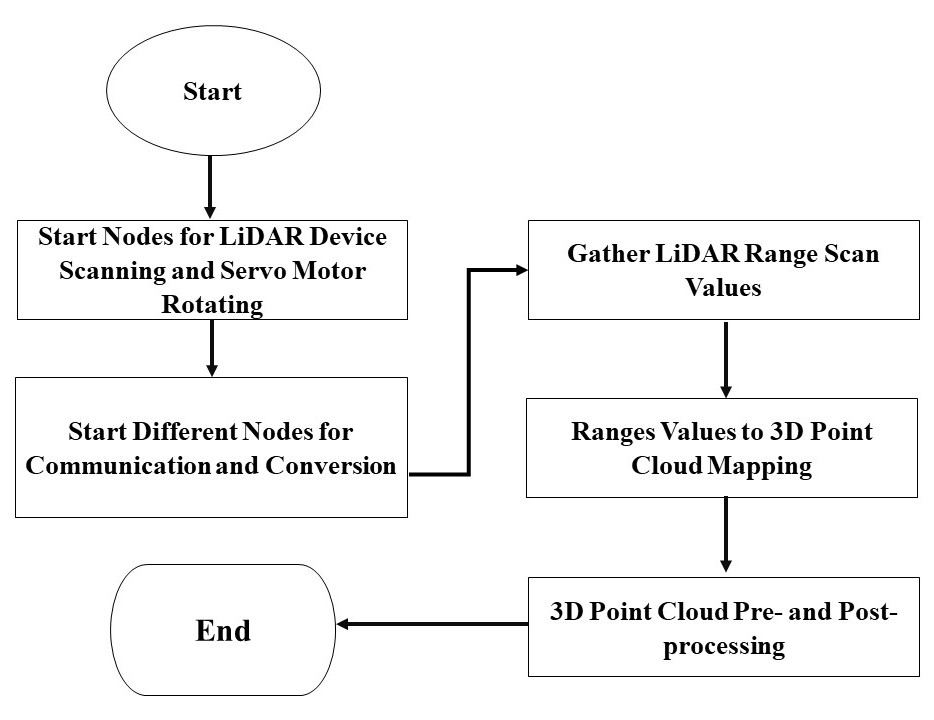
\includegraphics[width=0.9\textwidth]{Figures/scanning-to-pc-flow-chart}
	\caption{From Scanning to Mapped Point Cloud Data Flow Chart}
	\label{ch3:fig:scanning-to-pc-flow-chart}
\end{figure}

\begin{equation}
	\label{ch3:eq:x}
	x = \rho \cdot \sin(\theta) \cdot \cos(\phi)
\end{equation}
\begin{equation}
	\label{ch3:eq:y}
	y = \rho \cdot \sin(\theta) \cdot \sin(\phi)
\end{equation}
\begin{equation}
	\label{ch3:eq:z}
	z = \rho \cdot \cos(\theta)
\end{equation}

\subsubsection{Volume Measurement Process}
\label{ch3:sec:Volume Estimation}
An empty-space approach was used to measure the flour materials inside the storage bin. A simple representation of an empty-space approach is done following the concept discussed in section \ref{intro:sec:Conceptual Framework} where the 3D point cloud scanner system is placed at the top of the storage bin to scan the empty space and generate point cloud data. These point cloud data are processed to calculate the empty space volume using the Convex Hull method, specifically utilizing the Quickhull algorithm. The Quickhull algorithm computes the convex hull of the gathered point cloud data, enabling for volume estimation. Theoretically, as shown in equation \ref{ch4:eq:volume}, the volume of the flour materials is determined by subtracting the empty space volume from the bin's maximum volume capacity, a commonly used method in these studies \citet{raba2020,clar2022}.

\begin{figure}[H]
	\centering
	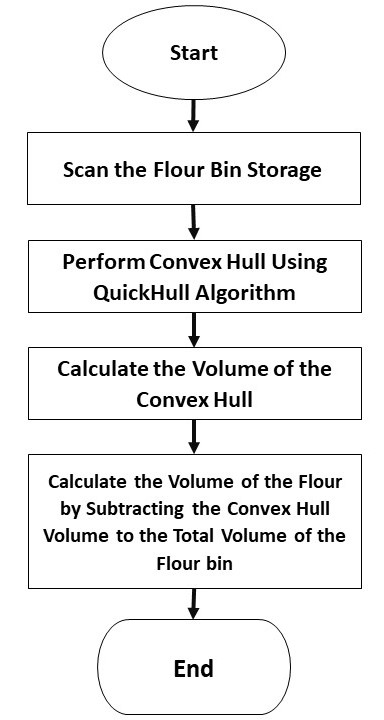
\includegraphics[width=0.5\textwidth, height=0.9\textwidth]{Figures/volume-estimation-process}
	\caption{Flow Chart of the System's Volume Measurement Process}
	\label{ch3:fig:volume-measurement-process}
\end{figure}

\begin{equation}
	\label{ch4:eq:volume}
	V_f = V_{max} - V_{empty}
\end{equation}

\begin{align*}
	 & \text{Where:}    &                                          \\
	 & V_f              & : \text{Volume of the flour materials}   \\
	 & V_{\text{max}}   & : \text{Total volume of the flour bin}   \\
	 & V_{\text{empty}} & : \text{Volume of the empty space}     &
\end{align*}

% \section{Web-based Application Development}
% This custom user interface based on web application is developed to used for the 3D-PCSS. The tools, framework and and resources of the system is discussed in this section.

% \subsection{}

% The user interface consider the following design and functionality, the UI should be:
% \begin{itemize}
% 	\item Intuitive and simple.
% 	\item Able to establish connection to the 3D-PCSS.
% 	\item Able to send command, display 3D point cloud data and volume measurement.
% \end{itemize}


\section{Web Application Development}
This section covers the process of developing the custom web application for the 3D point cloud scanner system.


% The user interface includes analysis of what data and value should be display in the UI, what tools, frameworks and library being used, what different section is consider in the dashboard. Lastly, what data is saved in the database. The analysis of the user interface requirements in this study considers the following functionalities:

% \begin{itemize}
% 	\item The user interface can able to connect to the system, check the connection from the system and view point cloud and measured volume data.
% 	\item Able to store the different measurement data.
% 	\item Has a dedicated section to visualize the stored data.
% \end{itemize}
\subsection{Different Tools and Framework}
The developed web application includes identifying the necessary tools and framework. These different tools and framework are essential for building the design and functionality of the UI. Table \ref{ch3:tab:tools-frameworks} outlines the various tools, frameworks, and libraries utilized in the implementation of the web application.

% \subsection{Tools and Frameworks}

\begin{table}[H]
	\centering
	\begin{threeparttable}
		\fullwidthcaption{Tools and Frameworks Used in the Web Application}
		\label{ch3:tab:tools-frameworks}
		\begin{tabular}{l p{9cm} }
			\toprule
			\textbf{Tool/Framework} & \textbf{Description/Functionality}                                                                                                                                                \\ \midrule
			jQuery                  & Used for simplifying JavaScript programming and DOM manipulation, jQuery is included via CDN for easy integration.                                                                \\ \midrule
			Three.js                & This JavaScript library is utilized for rendering 3D graphics in a web browser. It enables the display of the 3D point cloud viewer within the application.                       \\ \midrule
			EventEmitter2           & EventEmitter2 is employed for implementing event-driven programming, allowing efficient communication between different components of the application.                            \\ \midrule
			roslib.js               & roslib.js is utilized for connecting the web application to the Robot Operating System (ROS), enabling communication with ROS nodes and topics.                                   \\ \midrule
			Bootstrap               & The Bootstrap framework is employed for responsive design and styling of the user interface components. It ensures consistency and enhances the visual appeal of the application. \\ \midrule
			Chart.js                & This JavaScript library is used for creating interactive charts and graphs to visualize data. It enhances the user experience by providing intuitive data representation.         \\ \midrule
			ros3d.js                & ros3d.js is utilized for integrating ROS visualization capabilities into the web application. It facilitates the display of ROS topics such as point clouds and robot models.     \\ \bottomrule
		\end{tabular}
	\end{threeparttable}
\end{table}


These tools and frameworks collectively contribute to the functionality of the web application for the 3D Point Cloud Scanner System.

\subsection{Dashboard Development}
Analysis of the data and values to be displayed in the web application is conducted. This data and values are displayed in different section of the developed dashboard. The Web Application include storing of the measured volume coming from the system. The specific database used is MySQL which is running locally and retrieved to display in the dashboard.
% \subsection{Database Development}
% The Web Application include storing of the measured volume coming from the system. The database was running locally and retrieved to display in the dashboard.
\subsection{Overall System Integration}
\label{ch3:subsec:overall-system-integration}

Figure \ref{ch3:fig:web_app_connection} shows the process flow chart of the scanner system and web app. The flow illustrates the different processes, starting from powering the system, up to saving the measured volume to the database.

\begin{figure}[H]
	\centering
	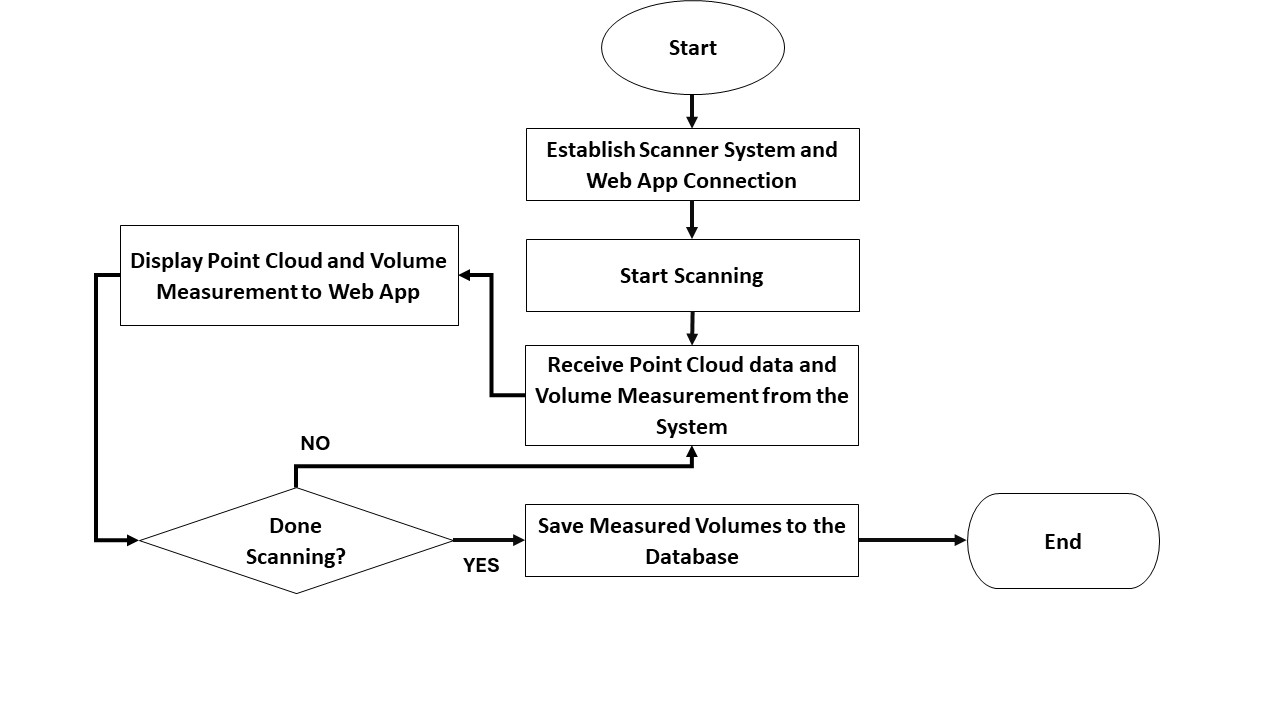
\includegraphics[width=1\textwidth]{Figures/process-flow}
	\caption{Process Flow Chart of Scanner System and Web App}
	\label{ch3:fig:web_app_connection}
\end{figure}

The connection between scanner system and web application uses a WebSocket communication protocol. This communication uses full-duplex channels to establish over a single TCP connection. It allows for less latency than typical HTTP connections when a client and server interact. Within the framework of ROS applications, WebSocket enables bi-directional, real-time communication, enabling servers to rapidly transmit updates to clients. The figure \ref{ch3:fig:websocket-connection} demonstrate the initialization of the Websocket communication between the web interface and the 3D-PCSS. The following step to establish this communication is explain below:

\begin{enumerate}
	\item \textbf{The Client Makes a Request:} The WebSocket client initiates the handshake by sending an connection request to the server.
	\item \textbf{The Server Accepts the Request:} If the server is willing to establish a WebSocket connection, it responds with an accept response that has a status code of 101 (Switching Protocols).
	\item \textbf{WebSocket Connection Established:} Once both the client and server have exchanged their handshake messages, the WebSocket connection is established. Data can now flow bidirectionally between the client and server over the single TCP connection.
\end{enumerate}

\begin{figure}[H]
	\centering
	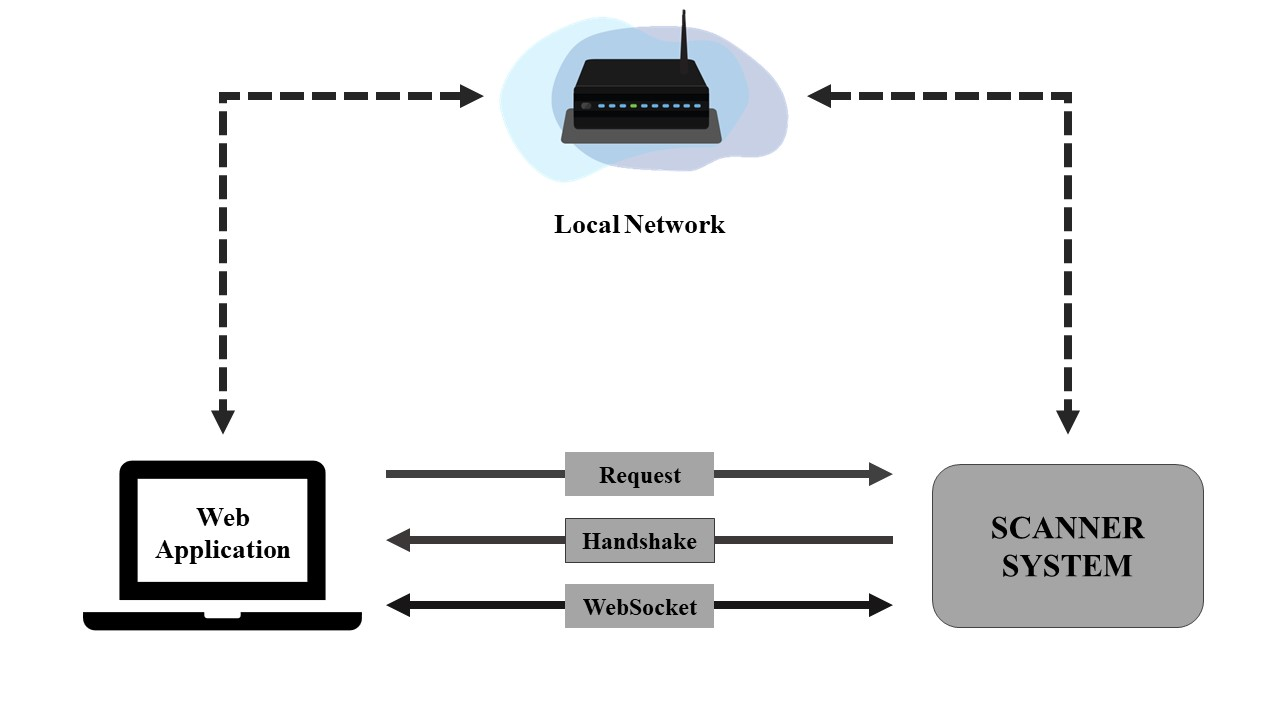
\includegraphics[width=0.9\textwidth]{Figures/websocket-connection}
	\caption{Communication Protocol of the Web Interface and the System}
	\label{ch3:fig:websocket-connection}
\end{figure}

\section{System Testing and Evaluation}
\label{ch3:sec:TestingAndEvaluation}

The study conducted different tests and evaluation to observe the accuracy and performance of the overall system. The testing methods involved calibration test and volume measurement test of the system.

% \subsection{Constructing of Storage Bin}
% \label{ch3:subsec:constructing-of-storage-bin}
% To test the performance and accuracy of the overall system, the study involves constructing a mock-up flour storage bin modeled after those commonly used in food manufacturing industries. The mock-up bin is designed to closely mimic the geometric shape and proportions of real storage bins used in practice. The CAD model design, shown in figure \ref{ch3:fig:cad_storage_bin}, serves as the guide for the physical construction. The design is composed of rectangular shape and conical frustum underneath. The CAD design of rectangular shape has a dimension of 2.5 meters in height, 0.5 meters in length, and 0.69 meters in width. The conical frustum, which is tapers from the base of the rectangular section, has a top radius of 0.21 meters, a bottom radius of 0.17 meters and height of 0.42 meters. The 3D-PCSS was placed at the top of created mock-up storage bin for test and evaluation.

% \begin{figure}[H]
% 	\centering
% 	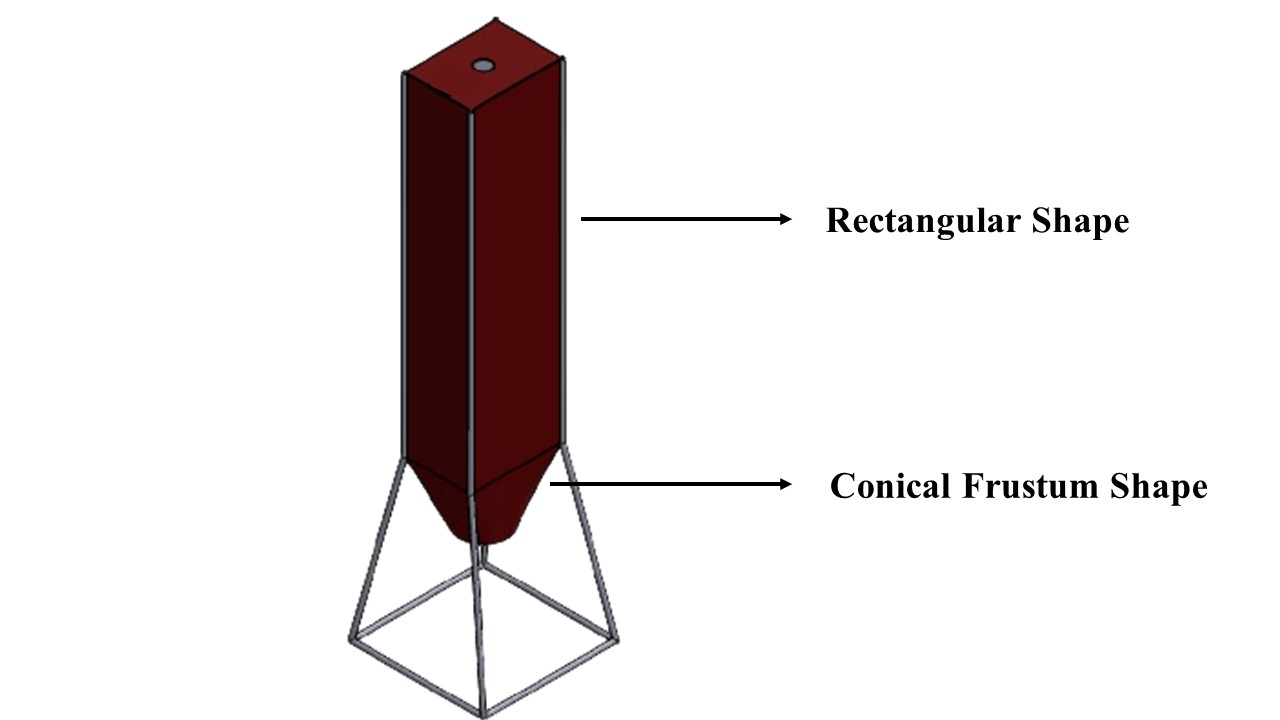
\includegraphics[width=1\textwidth]{Figures/cad_storage_bin}
% 	\caption{CAD Model Design of the Storage Bin}
% 	\label{ch3:fig:cad_storage_bin}
% \end{figure}

% \subsection{System Testing Methods}
% \label{ch3:subsec:system-testing-methods}
% The study conducted different tests to observe the accuracy and performance of the overall system. The testing methods involved laboratory test and actual field test of the system..

\subsection{LiDAR and Servo Calibration Test}
% \subsubsection{LiDAR Range and Servo Angle Test}
The purpose of the LiDAR and servo calibration test was to adjust the accuracy of the range values recorded and the rotating angle of the servo motor, which is crucial for ensuring that the system accurately captures the spatial data necessary for generating precise 3D point clouds. The calibration testing setup was done in the laboratory room, where the range values of the LiDAR device were calibrated using a known reference distance. The LiDAR was positioned at various distances from the reference object, and the measured range values were compared against the known distances. Similarly, the angle of rotation of the servo motor was calibrated to ensure accurate positioning by commanding the servo to specific angles and verifying its actual position using a calibration tool, with any discrepancies between commanded and actual angles corrected through calibration adjustments.
% \subsubsection{LiDAR Range Calibration}
% In this test, the range values of the LiDAR device were calibrated using a known reference distance. The LiDAR was positioned at various distances from the reference object, and the measured range values were compared against the known distances.
% \subsubsection{Servo Angle Calibration Test}
% The angle of rotation of the servo motor was calibrated to ensure accurate positioning. This involved commanding the servo to specific angles and verifying its actual position using a calibration tool. Any discrepancies between commanded and actual angles were corrected through calibration adjustments.

% \subsection{System Volume Measurement Calibration Test}
% \label{ch3:subsection:volume-measurement-test}
% The different volume measurement testing aimed to assess the accuracy and reliability of the 3D Point Cloud Scanner System in measuring the volume. This involved conducting different tests to evaluate the system's performance across different scenarios.

\subsection{System Volume Measurement Calibration Test}
\label{ch3:subsection:volume-measurement-test}

The calibration test aimed to assess the accuracy and reliability of the 3D Point Cloud Scanner System in measuring volume. This involved conducting various tests to evaluate the system's performance across different scenarios.

% \subsubsection{Testing Setup}
% \label{ch3:subsubsec:testing-setup}
% The testing setup involves constructing a mock-up flour storage bin. The mock-up flour storage bin is designed to closely mimic the geometric shape of the flour storage bins used in industry. The CAD model design, shown in figure \ref{ch3:fig:cad_storage_bin}, serves as the guide for the physical construction. The design is composed of rectangular shape and conical frustum underneath.

% The CAD design of rectangular shape has the following dimensions:
% \begin{itemize}
% 	\item Height: 2.5 meters
% 	\item Length: 0.5 meters
% 	\item Width: 0.69 meters
% \end{itemize}

% The conical frustum, which tapers from the base of the rectangular section, has the following dimensions:
% \begin{itemize}
% 	\item Top radius: 0.21 meters
% 	\item Bottom radius: 0.17 meters
% 	\item Height: 0.42 meters
% \end{itemize}

% Before the system was placed on top of the flour storage bin to conduct different testing procedures, the system was calibrated and adjusted based on acceptable accuracy.


% \begin{figure}[H]
% 	\centering
% 	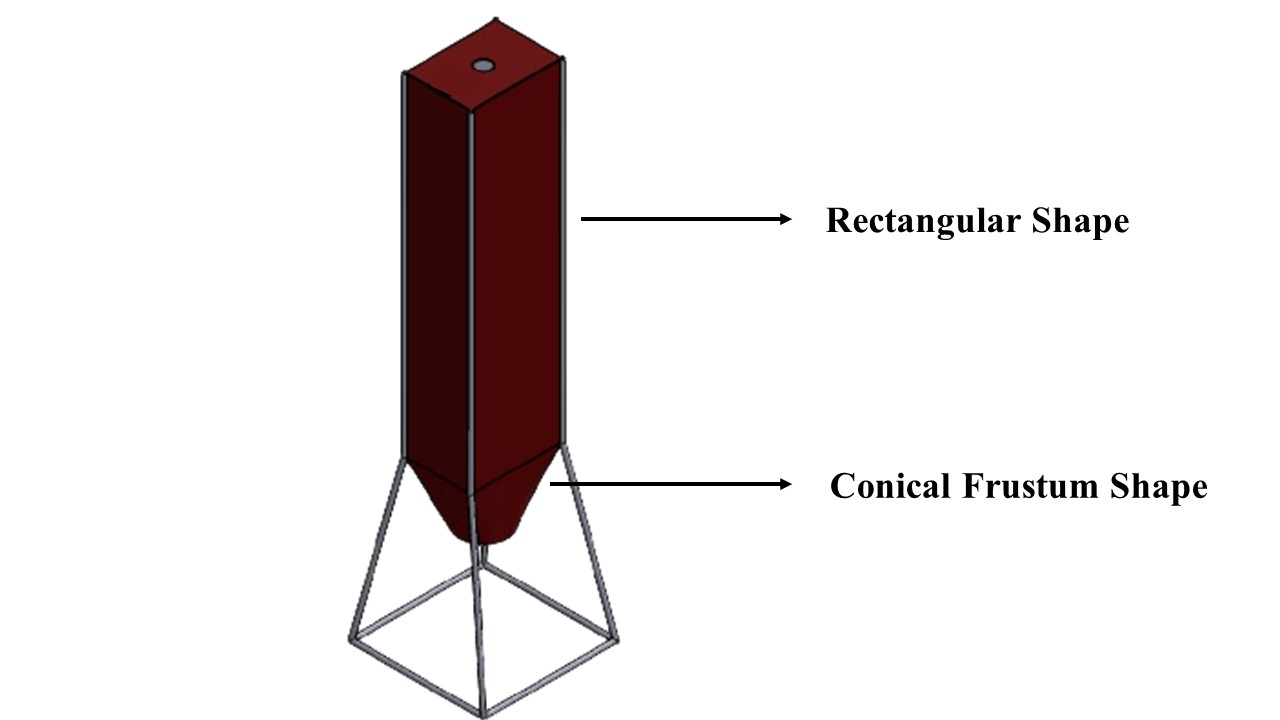
\includegraphics[width=1\textwidth]{Figures/cad_storage_bin}
% 	\caption{CAD Model Design of the Storage Bin}
% 	\label{ch3:fig:cad_storage_bin}
% \end{figure}

\subsubsection{Testing Setup}
\label{ch3:subsubsec:testing-setup}

The calibration test setup involved constructing a mock-up flour storage bin designed to closely mimic the geometric shape of the flour storage bins used in the industry. The CAD model design, shown in Figure \ref{ch3:fig
}, served as the guide for the physical construction. The design consisted of a rectangular shape with a conical frustum underneath.

The CAD design of the rectangular shape had the following dimensions:
\begin{itemize}
	\item Height: 2.5 meters
	\item Length: 0.5 meters
	\item Width: 0.69 meters
\end{itemize}

The conical frustum, which tapers from the base of the rectangular section, had the following dimensions:
\begin{itemize}
	\item Top radius: 0.21 meters
	\item Bottom radius: 0.17 meters
	\item Height: 0.42 meters
\end{itemize}

Before conducting different calibration test procedures, the system was calibrated and adjusted to minimize the error.
\begin{figure}[H]
	\centering
	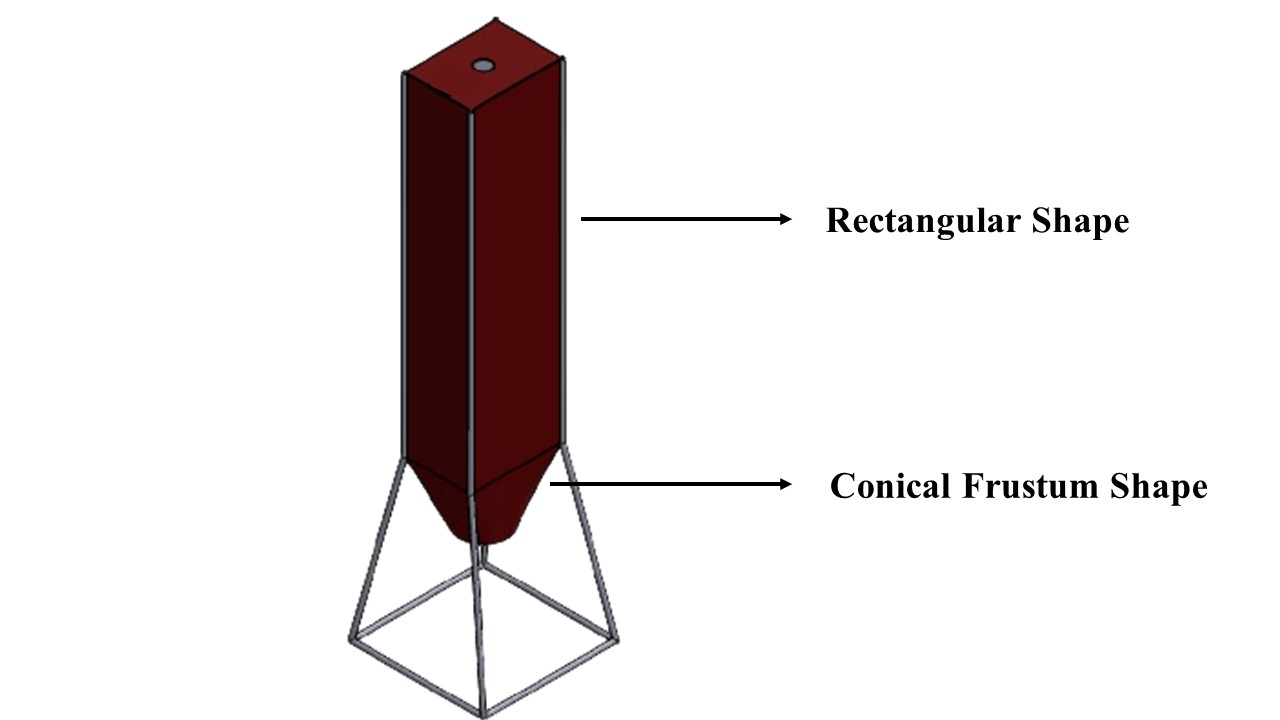
\includegraphics[width=1\textwidth]{Figures/cad_storage_bin}
	\caption{CAD Model Design of the Storage Bin}
	\label{ch3:fig
	}
\end{figure}

% \subsubsection{Empty Storage Volume Measurement}
% In this test, multiple scans of an empty storage bin to measure the total volume of the storage were conducted. The testing purposely scan the storage bin without flour materials inside. This involved performing 30 or more scanning trials. Before conducting the test, the actual total volume of flour storage bin was manually measured and calculated based on its actual geometric shapes and dimensions, this was done by using a measuring tool like steel tape measure.

\subsubsection{Empty Storage Volume Measurement Calibration}
\label{ch3:subsubsec:empty-storage-volume-measurement-calibration}
This calibration test involved performing multiple scans of an empty storage bin to measure its total volume. The purpose of this test was to scan the storage bin without any flour materials inside, ensuring an accurate baseline measurement. A total of 30 or more scanning trials were conducted. Before starting the test, the actual total volume of the flour storage bin was manually measured and calculated based on its geometric shapes and dimensions using a measuring tool like a steel tape measure.

% \subsubsection{Different Volume Quantity Measurement Calibration}
% \label{ch3:subsubsec:different-volume-measurement-test}

% This test involved filling the storage bin with flour materials of different volume quantity. A container with a known volume was used to ensure the precise quantification of the added flour top the storage bin for comparison with the system's measurements.

% Three specific volume quantity of the flour materials were filled in the storage bin. Additionally, to test the consistency of the system in measuring the volume with the same quantity, two different flour surface contours was conducted on each of the following test:

% \begin{enumerate}
% 	\item The storage bin was filled with 0.0594 $m^3$ of flour.
% 	\item The storage bin was filled with 0.4752 $m^3$ of flour.
% 	\item The storage bin was filled with 0.7128 $m^3$ of flour.
% \end{enumerate}

% The test comprised of 5 multiple scans for each of the two different surface contours, totaling 10 scans per test scenario.

\subsubsection{Different Volume Quantity Measurement Calibration}
\label{ch3:subsubsec:different-volume-measurement-test}

This calibration test involved filling the storage bin with different quantities of flour materials to assess the system's accuracy in measuring varying volumes. A container with a known volume was used to ensure precise quantification of the added flour for comparison with the system's measurements.

Three specific volumes of flour were tested:
\begin{enumerate}
	\item The storage bin was filled with 0.0594 $m^3$ of flour.
	\item The storage bin was filled with 0.4752 $m^3$ of flour.
	\item The storage bin was filled with 0.7128 $m^3$ of flour.
\end{enumerate}

To test the consistency of the system, each volume test included two different flour surface contours, with 5 multiple scans for each contour, totaling 10 scans per test scenario.

\subsubsection{Volume Measurement Using the System and Sounding Method Test}
To validate the accuracy and reliability of the 3D Point Cloud Scanner System, its volume measurements were compared with those obtained using the traditional sounding method. The traditional sounding method involves manually measuring the depth of the flour in the storage bin using a measuring tools such as tape measurement and calculating the volume based on the geometric shape and dimensions of the bin.

The comparison was conducted by filling the storage bin with a known volume of flour and measuring the volume using both methods. The specific steps were as follows:
\begin{enumerate}
	\item The storage bin was filled with a known volume of flour.
	\item The surface contour of the flour was adjusted into five different shapes.
	\item For each contour shape, the volume was measured using the system and traditional sounding method.
	\item The volume was then calculated based on the geometric shape and dimensions of the storage bin.
	\item The results from both methods were recorded and compared.
\end{enumerate}

% \begin{itemize}
% 	\item \textbf{Test Case 1: } In this test case, multiple scans of an empty storage bin were conducted. This involved performing 30 or more scanning trials to measure the total volume of the bin. Before conducting the test, the actual total volume of flour storage bin was manually measured and calculated based on its actual geometric shapes and dimensions, this was done by using a measuring tool like steel tape measure. By comparing the system's measured volume with the actual total volume of the storage bin, the baseline of its performance and accuracy in measuring the total volume of the flour bin could be identified. This baseline served as a reference point for subsequent testing.
% 	\item \textbf{Test Case 2: } The second test case involved filling the flour storage bin to various percentages of its total maximum volume. To accurately measure the volume of flour materials added to the bin, a container with a known volume was used for filling. This ensured precise quantification of the added flour for comparison with the system's measurements.

% 	      The following three specific percentage level of the bin were filled scanned by the system:

% 	      \begin{enumerate}
% 		      \item The storage bin was filled up to 5.8\% of its maximum capacity, with a known volume of 0.0594 cubic meters.
% 		      \item The storage bin was filled up to 47.2\% of its maximum capacity, with a known volume of 0.4752 cubic meters.
% 		      \item The storage bin was filled up to 70.37\% of its maximum capacity, with a known volume of 0.7128 cubic meters.
% 	      \end{enumerate}

% 	      The test comprised of 5 multiple scans for each of the two different surface contours, totaling 10 scans per test scenario. The objective was to assess the system's performance and measurement accuracy at different fill levels. Additionally, scanning with different surface contours aimed to evaluate the consistency of the system's measurements for same volumes value but different surface contour.
% \end{itemize}

% \subsubsection{Test Case 1: Empty Storage Bin Scanning}

% In this test case, multiple scans of an empty storage bin were conducted. This involved performing 30 or more scanning trials to measure the total volume of the bin. Before conducting the test, the actual total volume of flour storage bin was manually measured and calculated based on its actual geometric shapes and dimensions, this was done by using a measuring tool like steel tape measure. By comparing the system's measured volume with the actual total volume of the storage bin, the baseline of its performance and accuracy in measuring the total volume of the flour bin could be identified. This baseline served as a reference point for subsequent testing.

% \subsubsection{Test Case 2: Filling the Storage Bin with Known Volume}
% \label{ch3:subsec:test-case-2}

% The second test case involved filling the flour storage bin to various percentages of its total maximum volume. To accurately measure the volume of flour materials added to the bin, a container with a known volume was used for filling. This ensured precise quantification of the added flour for comparison with the system's measurements.

% The following three specific percentage level of the bin were filled scanned by the system:

% %Each with different percentages of the storage bin's maximum capacity, along with known volumes and conducted a two different flour surface contour:

% \begin{enumerate}
% 	\item The storage bin was filled up to 5.8\% of its maximum capacity, with a known volume of 0.0594 cubic meters.
% 	\item The storage bin was filled up to 47.2\% of its maximum capacity, with a known volume of 0.4752 cubic meters.
% 	\item The storage bin was filled up to 70.37\% of its maximum capacity, with a known volume of 0.7128 cubic meters.
% \end{enumerate}

% The test comprised of 5 multiple scans for each of the two different surface contours, totaling 10 scans per test scenario. The objective was to assess the system's performance and measurement accuracy at different fill levels. Additionally, scanning with different surface contours aimed to evaluate the consistency of the system's measurements for same volumes value but different surface contour.

%These different test cases were designed to assess the accuracy and performance of the overall system.

% These test cases were crucial in evaluating the accuracy and performance of the system under different conditions.
% \subsection{Evaluation of the System}
% \label{ch3:subsec:Evaluation of the System}
% Based on the conducted different testing mentioned in \ref{ch3:subsec:Different Testing Procedure}, the researcher will evaluate the conducted testing based on the volume of scanned data. System in the following evaluation

% To evaluate the testing \ref{ch3:first}, the researcher will measure the accuracy of the system by comparing the estimated volume of the system  with the actual volume of the different shape of the bin, calculate the error percentage for each trial and assess the over all precision of the system. Table \ref{ch3:tab:Testing 1} shows the sample comparison of the testing.

% \begin{table}[H]
% 	\caption{Testing \ref{ch3:first}}
% 	\label{ch3:tab:Testing 1}
% 	\centering
% 	\begin{tabular}{|c|c|c|c|}
% 		\hline
% 		% First row
% 		Flour bin Shape & Actual Volume (\si{mm^3}) & Scanned Volume (\si{mm^3}) & Error (\%) \\
% 		\hline
% 		\multicolumn{4}{|c|}{Trial 1}                                                         \\
% 		\hline
% 		% Second row
% 		Cube            & -                         & -                          & -          \\
% 		\hline
% 		% Third row
% 		Cylinder        & -                         & -                          & -          \\
% 		\hline
% 		\multicolumn{4}{|c|}{Trial 2}                                                         \\
% 		\hline
% 		Cube            & -                         & -                          & -          \\
% 		\hline
% 		% Third row
% 		Cylinder        & -                         & -                          & -          \\
% 		\hline
% 	\end{tabular}
% \end{table}

% Testing \ref{ch3:second} will be evaluated from the testing \ref{ch3:first} based on the number of point cloud acquired of both testing, and compare it. Basically, the testing \ref{ch3:second} will acquired more point cloud compared to testing \ref{ch3:first} due to multi-echo or multiple returning from the dust and the flour bin.

% In testing \ref{ch3:third} and \ref{ch3:fourth}, the researcher will place flour materials inside the bin with different surface shape and perform volume estimation. After the volume estimation, the researcher will generate dust, scan the bin, perform volume estimation and compare it to the result of the testing \ref{ch3:third}. The sample result of testing \ref{ch3:third} and \ref{ch3:fourth} is shown in table

% \begin{table}[H]
% 	\caption{Testing 3 and 4}
% 	\label{ch3:tab:Testing 3 and 4}
% 	\centering
% 	\begin{tabular}{|c|p{0.27\linewidth}|p{0.26\linewidth}|p{0.2\linewidth}|}
% 		\hline
% 		% First row
% 		Flour bin Shape & Scanned Volume (without dust) & Scanned Volume (with dust) & Error (\%) \\
% 		\hline
% 		\multicolumn{4}{|c|}{Surface Shape 1}                                                     \\
% 		\hline
% 		% Second row
% 		Cube            & -                             & -                          & -          \\
% 		\hline
% 		% Third row
% 		Cylinder        & -                             & -                          & -          \\
% 		\hline
% 		\multicolumn{4}{|c|}{Surface Shape 2}                                                     \\
% 		\hline
% 		Cube            & -                             & -                          & -          \\
% 		\hline
% 		% Third row
% 		Cylinder        & -                             & -                          & -          \\
% 		\hline
% 	\end{tabular}
% \end{table}

\subsection{System Evaluation}
The system evaluation phase aimed to assess the overall performance and effectiveness of the system in fulfilling its intended objectives. This evaluation involved analyzing various aspects of the system, including the performance of the LiDAR sensor, the accuracy of servo motor control, and the reliability of volume measurement calculations.

\subsubsection{LiDAR Range Evaluation}
After the calibration of th device, any discrepancies or deviations from expected values are analyzed to identify and adjusted. Performance assessment of LiDAR range involves conducting range measurements across different distances. The measured range values are compared against reference distances to evaluate accuracy and precision.
Sa lidar range parameter is distances in meters,
\subsubsection{Servo Angle Evaluation}
The commanded and actual angles are compared to determine positional accuracy and repeatability. Additionally, the system's responsiveness to servo control commands is evaluated to assess its overall performance in angle adjustment and positioning tasks.
servo angle parameter in degree.

\subsubsection{Empty Storage Bin Volume Measurement Evaluation}
In the evaluation of the Empty Storage Bin Volume Measurement test, the performance and accuracy of the system were assessed using several metrics. Firstly, the Mean Absolute Percentage Error (MAPE) was calculated by comparing the system's measured volume with the actual total volume of the storage bin. The average measured volume of the system was determined, considering the associated uncertainty. Lastly, the precision of the system was evaluated based on the closeness of the measured data points.
\subsubsection{Different Volume Quatity Measurement Evaluation}
In the evaluation of the Different Volume Measurement Test, the performance of the system in accurately measuring flour volumes of varying quantities was assessed using multiple evaluation metrics. The average measured volume with uncertainty was calculated for each test scenario. Moreover, the Mean Absolute Error (MAE) was used to evaluate the accuracy of the system's measurements across the different volume quantities. Lastly, the performance of the system in terms of precision across the different volume quantity was assessed.

\subsubsection{Comparison Evaluation of the System and Sounding Method}
In this comparison evaluation, the system's volume measurements were compared with those obtained using the traditional sounding method. A known volume of flour was filled into the storage bin, and the surface contour was adjusted into five different shapes. For each contour shape, volume measurements were taken using both the 3D Point Cloud Scanner System and the traditional sounding method. The accuracy and reliability of the system were evaluated by comparing the measured volumes from both methods and calculating the percentage differences. This comparison aimed to highlight the system's overall performance over sounding method.

% To evaluate the system's performance and measured volume based on the test methods, a comparative analysis was conducted between the actual volume and the measured volume obtained during the testing.

% The Mean Absolute Percentage Error (MAPE) was used to identify the average percentage difference between the measured volume of the system relative to the actual volume. This method would suggest how closely the system's measurements align with the actual values.

% Standard Deviation (SD) was also used to identify the dispersion of the system's measured volume. The observation of SD suggests how clustered the measurement of the system.  Overall, these statistical tools were essential for evaluating system's accuracy and precision in measuring the volume relative to the actual volume.